\documentclass[11pt,letterpaper]{article}

\addtolength{\oddsidemargin}{-.875in}
\addtolength{\evensidemargin}{-.875in}
\addtolength{\textwidth}{1.75in}

\addtolength{\topmargin}{-.875in}
\addtolength{\textheight}{1.75in}

\usepackage[utf8]{inputenc}
\usepackage{caption} % for table captions
\usepackage{amsmath} % for multi-line equations and piecewises
\DeclareMathOperator{\sign}{sign}
\usepackage{graphicx}
\usepackage{relsize}
\usepackage{xspace}
\usepackage{verbatim} % for block comments
\usepackage{subcaption} % for subfigures
\usepackage{enumitem} % for a) b) c) lists
\newcommand{\Cyclus}{\textsc{Cyclus}\xspace}%
\newcommand{\Cycamore}{\textsc{Cycamore}\xspace}%
\newcommand{\deploy}{\texttt{d3ploy}\xspace}%
\newcommand{\Deploy}{\texttt{D3ploy}\xspace}%
\usepackage{tabularx}
\usepackage{color}
\usepackage{multirow}
\usepackage{float} 
\usepackage[acronym,toc]{glossaries}
\newacronym{ANL}{ANL}{Argonne National Laboratory}
\newacronym{B4C}{B4C}{boron carbide}
\newacronym{BC}{BC}{boundary condition}
\newacronym{BOC}{BOC}{beginning of equilibrium cycle}
\newacronym{BSD}{BSD}{Berkeley Software Distribution}
\newacronym{BWR}{BWR}{Boiling Water Reactor}
\newacronym{CAISO}{CAISO}{California ISO}
\newacronym{CEA}{CEA}{Commissariat a l'Energie Atomique}
\newacronym{CFD}{CFD}{computational fluid dynamics}
\newacronym{CO2}{CO$_2$}{carbon dioxide}
\newacronym{CR}{CR}{control rod}
\newacronym{CRP}{CRP}{Coordinated Research Project}
\newacronym{CZP}{CZP}{Cold Zero Power}
\newacronym{DCC}{DCC}{depressurized conduction cool-down}
\newacronym{DOE}{DOE}{Department of Energy}
\newacronym[\glslongpluralkey={degrees of freedom}]{DoF}{DoF}{degree of freedom}
\newacronym{EOC}{EOEC}{end of equilibrium cycle}
\newacronym{FCEV}{FCEV}{Fuel Cell Electric Vehicle}
\newacronym{FDM}{FDM}{Finite Difference Method}
\newacronym{FEM}{FEM}{Finite Element Method}
\newacronym{FVM}{FVM}{Finite Volume Method}
\newacronym{FSV}{FSV}{Fort St. Vrain}
\newacronym[\glslongpluralkey={greenhouse gases}]{GHG}{GHG}{greenhouse gas}
\newacronym{GRS}{GRS}{Gesellschaft für Anlagen und Reaktorsicherheit}
\newacronym{H2}{H$_2$}{hydrogen}
\newacronym{He}{He}{helium}
\newacronym{HFP}{HFP}{Hot Full Power}
\newacronym{HPCC}{HPCC}{high pressure conduction cool-down}
\newacronym{HTE}{HTE}{High-Temperature Electrolysis}
\newacronym{HTGR}{HTGR}{High-Temperature Gas-Cooled Reactor}
\newacronym{HTR}{HTR}{High Temperature Reactor}
\newacronym{HTTR}{HTTR}{High Temperature Test Reactor}
\newacronym{HZDR}{HZDR}{Helmholtz-Zentrum Dresden-Rossendorf}
\newacronym{IAEA}{IAEA}{International Atomic Energy Agency}
\newacronym{icap}{iCAP}{Illinois Climate Action Plan}
\newacronym{INL}{INL}{Idaho National Laboratory}
\newacronym{IPyC}{IPyC}{inner pyrolytic carbon}
\newacronym{JFNK}{JFNK}{Jacobian-Free Newton-Krylov}
\newacronym{KAERI}{KAERI}{Korea Atomic Energy Research Institute}
\newacronym{Keff}{K$_{eff}$}{multiplication factor}
\newacronym{LBP}{LBP}{Lumped Burnable Poison}
\newacronym{LGPL}{LGPL}{Lesser GNU Public License}
\newacronym{LOCA}{LOCA}{loss of coolant accident}
\newacronym{LPCC}{LPCC}{low pressure conduction cool-down}
\newacronym{LTE}{LTE}{Low-Temperature Electrolysis}
\newacronym{LWR}{LWR}{Light Water Reactor}
\newacronym{MC}{MC}{Monte Carlo}
\newacronym{MHTGR}{MHTGR}{Modular High-Temperature Gas-Cooled Reactor}
\newacronym{MOC}{MOC}{middle of equilibrium cycle}
\newacronym{MOOSE}{MOOSE}{Multi-physics Object-Oriented Simulation Environment}
\newacronym{MPI}{MPI}{Message Passing Interface}
\newacronym{MSR}{MSR}{Molten Salt Reactor}
\newacronym{MTD}{MTD}{Champaign-Urbana Mass Transit District}
\newacronym{NEA}{NEA}{Nuclear Energy Agency}
\newacronym{NEM}{NEM}{Nodal Expansion Method}
\newacronym{NGNP}{NGNP}{Next Generation Nuclear Power}
\newacronym{NRC}{NRC}{Nuclear Regulatory Commission}
\newacronym{NSC}{NSC}{Nuclear Science Committee}
\newacronym{OECD}{OECD}{Organisation for Economic Co-operation and Development}
\newacronym{OPyC}{OPyC}{outer pyrolytic carbon}
\newacronym{ORNL}{ORNL}{Oak Ridge National Laboratory}
\newacronym{OS}{OS}{Operator-Splitting}
\newacronym{PBMR}{PBMR}{Pebble Bed Modular Reactor}
\newacronym{PDE}{PDE}{Partial Differential Equation}
\newacronym{PMR}{PMR}{Prismatic Modular Reactor}
\newacronym{PV}{PV}{photovoltaics}
\newacronym{RSC}{RSC}{Reserve Shutdown Control}
\newacronym{RSD}{RSD}{Relative Standard Deviation}
\newacronym{SD}{SD}{Standard Deviation}
\newacronym{SI}{SI}{Sulfur-Iodine}
\newacronym{SiC}{SiC}{silicon carbide}
\newacronym{SMR}{SMR}{Small Modular Reactor}
\newacronym{SNU}{SNU}{Seoul National University}
\newacronym{SOEC}{SOEC}{Solid Oxide Electrolysis Cells}
\newacronym{TIP}{TIP}{transverse integration procedure}
\newacronym{TRISO}{TRISO}{Tristructural Isotropic}
\newacronym{UIUC}{UIUC}{University of Illinois at Urbana-Champaign}
\newacronym{UNIST}{UNIST}{Ulsan National Institute of Science and Technology}
\newacronym{UK}{UK}{United Kingdom}
\newacronym{UMICH}{UMICH}{University of Michigan}
\newacronym{US}{US}{United States}
\newacronym{VHTR}{VHTR}{Very High Temperature Gas Cooled Reactor}
%\newacronym{<++>}{<++>}{<++>}
%\newacronym{<++>}{<++>}{<++>}

\definecolor{bg}{rgb}{0.95,0.95,0.95}
\newcolumntype{b}{X}
\newcolumntype{f}{>{\hsize=.15\hsize}X}
\newcolumntype{s}{>{\hsize=.5\hsize}X}
\newcolumntype{m}{>{\hsize=.75\hsize}X}
\newcolumntype{r}{>{\hsize=1.1\hsize}X}
\usepackage{titling}
\usepackage[hang,flushmargin]{footmisc}
\renewcommand*\footnoterule{}
\usepackage{tikz}

\usetikzlibrary{shapes.geometric,arrows}
\tikzstyle{process} = [rectangle, rounded corners, 
minimum width=1cm, minimum height=1cm,text centered, draw=black, 
fill=blue!30]
\tikzstyle{arrow} = [thick,->,>=stealth]

\graphicspath{}

\begin{document}

\section{Introduction}

% The energy problem
Energy is one of the strongest contributors to economic growth.
In the future, economies will continue to grow, populations will do so too, and their energy demand will accompany such growth \cite{burke_impact_2018} \cite{el-shafie_hydrogen_2019}.
Meeting these future needs requires the development of clean energy sources as environmental concerns continue to rise.

As seen in Figure \ref{fig:ghg}, electricity generation was one of the economic sectors that released the most \glspl{GHG} in the \gls{US} in 2017.
As \gls{CO2} is the main component in \glspl{GHG}, decarbonizing electricity generation will allow us to meet the increases in energy demand and address the environmental concerns at the same time.

\begin{figure}[htbp!]
	\centering
	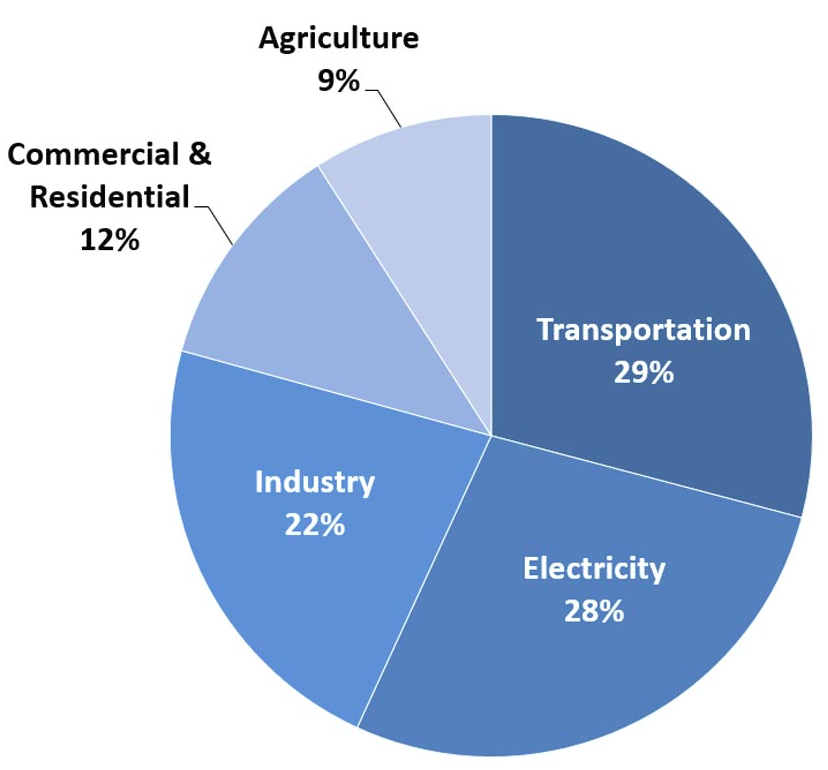
\includegraphics[width=0.6\linewidth]{figures/total-ghg-2017.png}
	\hfill
	\caption{Total \gls{US} \gls{GHG} emissions by economic Sector in 2017. Image reproduced from \cite{us_epa_sources_2020}.}
	\label{fig:ghg}
\end{figure}

% word on solar energy and the duck curve
To address these concerns, utility companies are relying more and more on renewable energy resources, such as wind and solar \cite{ming_resource_2019}.
However, high solar adoption creates a challenge.
The need for electricity generators to quickly ramp up increases when the sun sets and the contribution from the \gls{PV} falls \cite{us_department_of_energy_confronting_2017}.
The "duck curve" (or duct chart) depicts this phenomenon, Figure \ref{fig:duck}.
The \gls{CAISO} developed the duck curve to illustrate the net load of the grid \cite{bouillon_prepared_2014}.
We define the net load as the difference between forecasted load and expected electricity production from solar.

Moreover, the duck curve reveals another issue.
Over-generation may occur during the middle of the day and high-levels of non-dispatchable generation may exacerbate the situation.
As a consequence, the market would experience sustained zero or negative prices during the middle of the operating day \cite{bouillon_prepared_2014}.

\begin{figure}[htbp!]
	\centering
	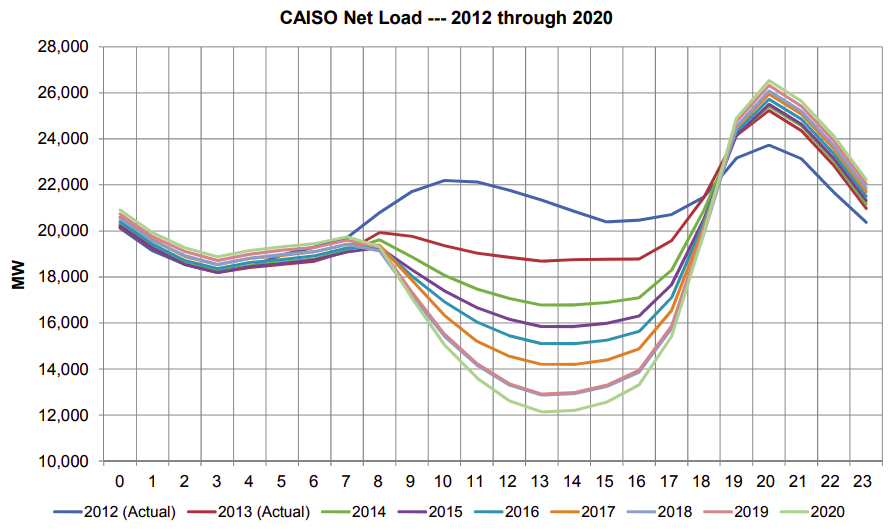
\includegraphics[width=1.0\linewidth]{figures/caiso-duck.png}
	\hfill
	\caption{The duck curve. Image reproduced from \cite{bouillon_prepared_2014}.}
	\label{fig:duck}
\end{figure}

% solutions to the duck curve
The simplest solution to a demand ramp up is to increase dispatchable generation, resources with fast ramping and fast starting capabilities such as natural gas and coal \cite{bouillon_prepared_2014}, and, consequently, decrease non-dispatchable generation, such as geothermal, nuclear, and hydro.
Nonetheless, an approach like this is not consistent with the goal of reducing carbon emissions.
Hence, our focus drifts to other potential low-carbon solutions, like nuclear generation and electricity storage by means of \gls{H2} production.

% Transportation problem
Unfortunately, a carbon neutral electric grid will be insufficient to halt climate change because transportation is a big contributor to \gls{GHG} emissions.
As seen in Figure \ref{fig:ghg}, transportation released the most \glspl{GHG} in the \gls{US} in 2017. Thus, decarbonizing transportation underpins global carbon reduction.

One possible strategy is to develop a hydrogen economy, as Japan is currently doing.
Japan's strategy rests on the firm belief that \gls{H2} can be a decisive response to its energy and climate challenges.
It could foster deep decarbonization of the transport, power, industry, and residential sectors while strengthening energy security \cite{nagashima_japans_2018}.
In the transportation sector, Japan is planning to deploy fuel cell vehicles, trucks, buses, trains, and ships.

Although \gls{H2} technologies do not release CO$_2$, any \gls{H2} production method is only as carbon-free as the source of energy it relies on (electric, heat, or both).
Nuclear reactors present a clean energy option to manufacture \gls{H2}.

The \gls{UIUC} is leading by example and actively working to reduce \gls{GHG} emissions on its campus produced by both economic sectors, electricity generation and transportation (among other sectors).
In pursuance of those efforts, the university has developed a climate action plan described in the following section.

\section{\gls{UIUC} case}
% ICAPP
In 2008, \gls{UIUC} signed the American College and University Presidents' Climate Commitment, formally committing to become carbon neutral as soon as possible, no later than 2050.
The university developed the first \gls{icap} in 2010 as a comprehensive roadmap toward a sustainable campus environment \cite{university_of_illinois_at_urbana-champaign_illlinois_2015}.
The \gls{icap} defines a list of goals, objectives, and potential strategies for the following six topical areas.

\begin{itemize}
	\item Energy Conservation and Building Standards:
\end{itemize}
This area focuses on maintaining or reducing campus gross square footage, strengthen centralized conservation efforts, and engage the campus community in energy conservation.

\begin{itemize}
	\item Energy Generation, Purchasing, and Distribution:
\end{itemize}
This area directs its efforts towards the exploration of 100\% clean campus energy options.
This includes the expansion of on-campus solar energy production, the expansion of the purchase of clean energy from low-carbon energy sources, and the offset of all emissions from the National Petascale Computing Facility.

\begin{itemize}
	\item Transportation:
\end{itemize}
This area comprises the efforts on reducing air travel emissions, Urbana-Champaign campus fleet emissions, study scenarios for complete conversion of the campus fleet to renewable fuels, and implementing the Campus Bike Plan.

\begin{itemize}
	\item Water and Stormwater:
\end{itemize}
This area focuses on improving water efficiency of cooling towers, perform a water audit to establish water conservation targets, determine upper limits for water demand by end-use, and implement pilot projects to showcase the potential of water and stormwater reuse.

\begin{itemize}
	\item Purchasing, Waste, and Recycling:
\end{itemize}
This area attempts to standardize the purchases of office paper, cleaning products, computers, other electronics, and freight delivery services. It also attempts to fomenting recycling by reducing nondurable goods purchases and reducing municipal solid waste going to landfills.

\begin{itemize}
	\item Agriculture, Land Use, Food, and Sequestration:
\end{itemize}
This area will perform a comprehensive assessment of \gls{GHG} emissions from agricultural operations, and develop a plan to reduce them, implement a project that examines the food service carbon footprint for Dining, and increase carbon sequestration in campus soils.

% Description of current grid ??
% Description of current fleet ??

\section{Objectives}

As mentioned earlier, we place our attention on two topics: electricity generation and transportation.
Consequently, the objective of this work aligns with the efforts in two of the six target areas defined on the \gls{icap} by turning our attention to electricity generation and transportation in the \gls{UIUC} campus.

Regarding electricity generation, our analysis focuses on the \gls{UIUC} grid.
One of the objectives of the \gls{icap} is the expansion of on-campus solar energy production.
As described earlier, an excess of solar energy integration to the grid makes the duck curve phenomenon likely to occur.
The present work studies the magnitude of the duck curve in \gls{UIUC} grid.
As noted earlier, the duck curve reveals a risk of over-generation due to high levels of non-dispatchable capacity.
To mitigate this issue, we propose to use the over-generated energy to manufacture \gls{H2}.
As one of the objectives of the \gls{icap} is the exploration of 100\% clean campus energy options, we chose a nuclear reactor to be one of the main sources of energy.
With the duck curve magnitude determined and an a reactor size chosen, the next step is to quantify how much \gls{H2} our method is able to produce.
Section \ref{sec:hydro} discusses a few hydrogen production methods considered for our analysis.
The last step determines how much electricity we would generate using the \gls{H2} produced.

Regarding transportation, we study the complete conversion to \glspl{FCEV} of the \gls{UIUC} fleet that works on campus.
This objective aligns with the interests of the \gls{icap}.
Additionally, the analysis includes the complete conversion of the \gls{MTD} fleet as well.
The first step is to determine the fuel consumed by both fleets and how much \gls{H2} enables the complete conversion of the fleets.
Finally, we consider a few reactor designs and analyze which of them could produce enough \gls{H2} to fulfill both fleet requirements.

Both studies propose the same solution, a nuclear reactor coupled to a hydrogen plant.
In terms of electricity generation, this solution will decrease the need for dispatchable sources and, consequently, reduce the carbon emissions of the electricity generation sector.
In terms of transportation, it will eliminate carbon emissions completely.

%Mention the choice of reactor
In both analysis, many reactor choices can satisfy our needs.
It could be one Microreactor, a series of Microreactors, or a \gls{SMR}.
Section \ref{sec:reactors} discusses their characteristics.

\section{Hydrogen production methods}
\label{sec:hydro}

This section introduces some hydrogen production processes.
The following subsections describe the energy requirements of some of the methods that could be coupled to a nuclear reactor.

\begin{itemize}
	\item Steam-Methane Reforming:
\end{itemize}

Steam reforming is a catalytic process that involves a reaction between natural gas (or other light hydrocarbons) and steam.
The result of a series of reactions is a mixture of hydrogen, carbon monoxide, carbon dioxide, and water.
The first reforming step catalytically reacts methane with steam to form hydrogen and carbon monoxide in an endothermic reaction.
A second reaction, an exothermic reaction, shifts the carbon monoxide with steam to form additional hydrogen and carbon dioxide.
Finally, an adsorption process could remove the carbon dioxide \cite{harper_us_2012}.
This process is currently the least expensive way to produce hydrogen \cite{doe_office_of_energy_efficiency_and_renewable_energy_hydrogen_2020}.

A \gls{HTGR} can substitute the natural gas burning furnaces as a heat source.
This approach reduces the \gls{CO2} emissions to the atmosphere in large quantities.
Nevertheless, due to the nature of the chemical reforming and shifting processes, this method still needs a natural gas feedstock \cite{yildiz_efficiency_2006}. 
Consequently, the method still emits \gls{CO2}, unless it includes a sequestration method.
A sequestration process complicates the plant layout and makes the process more expensive.
For this reason, we will not include this method in the analysis.
Further studies could consider it.

\begin{itemize}
	\item Coal Gasification:
\end{itemize}

The gasification of coal is one method that can produce power, liquid fuels, chemicals, and hydrogen.
Specifically, reacting coal with oxygen and steam under high pressures and temperatures forms a synthesis gas, a mixture consisting primarily of carbon monoxide and hydrogen \cite{doe_office_of_energy_efficiency_and_renewable_energy_hydrogen_2020}.
After removing the impurities from the synthesis gas, the water-gas shift reaction produces additional hydrogen and carbon dioxide form the carbon monoxide in the gas mixture.
A separation system removes the hydrogen.
This method still emits \gls{CO2} requiring a carbon sequestration system. 
We will not consider this process in the analysis.

\begin{itemize}
	\item Electrolysis: 
\end{itemize}

The electrolysis of water is a well-known method whose commercial use began in 1890.
This process produces approximately a 4\% of \gls{H2} worldwide.
The process is ecologically clean because it does not emit \glspl{GHG}, and the oxygen
produced has further industrial applications.
However, in comparison with other methods, electrolysis is a highly energy-demanding technology 
\cite{kalamaras_hydrogen_2013}.

Three electrolysis technologies exist.
Alkaline-based is the most common, the most developed, and the lowest in capital cost.
It has the lowest efficiency and, therefore, the highest electrical energy cost.
Proton exchange membrane electrolyzers are more efficient but more expensive than Alkaline electrolyzers.
\gls{SOEC} electrolyzers are the most electrically efficient but the least developed.
\gls{SOEC} technology has challenges with corrosion, seals, thermal cycling, and chrome migration \cite{kalamaras_hydrogen_2013}.
As the first two technologies work with liquid water and the latter requires high temperature steam, we will refer to the first two as \gls{LTE} and the latter as \gls{HTE}.

\begin{itemize}
	\item Thermo-chemical Water Splitting:
\end{itemize}

Thermochemical water-splitting is the conversion of water into hydrogen and oxygen by a series of thermally driven chemical reactions.
The direct thermolysis of water requires temperatures in excess of 2500 $^{\circ}$C for significant hydrogen generation.
At this temperature, the process is able to decompose a 10\% of the water.
A thermochemical water-splitting cycle accomplishes the same overall result using much lower temperatures.

In \cite{brown_high_2003}, General Atomics, Sandia National Laboratories, and the University of Kentucky compared 115 cycles that would use high temperature heat from an advanced nuclear reactor.
The reports specifies a set of objective screening criteria used to rate each cycle.
The highest scoring method was the \gls{SI} Cycle.

In 1978 and 1980, the process was coupled to a nuclear reactor.
The latter flowsheet indicated that hydrogen could be produced at 52\% efficiency.
This is the highest efficiency reported for any water-splitting process, based on an integrated flowsheet \cite{brown_high_2003}.

\begin{itemize}
	\item Photobiological processes:
\end{itemize}

In photolytic biological systems, microorganisms—such as green microalgae or cyanobacteria—use sunlight to split water into oxygen and hydrogen.
Challenges for this pathway include low rates of hydrogen production, low solar-to-hydrogen efficiency, and the fact that splitting water also produces oxygen \cite{doe_office_of_energy_efficiency_and_renewable_energy_hydrogen_2020}.
The latter inhibits the hydrogen production reaction and can be a safety issue.
All these challenges make it a commercially unviable pathway at this time.
We will not consider this method for the analysis.

\subsection{Electrolysis}

Water electrolysis converts electric and thermal energy into chemical energy stored in hydrogen \cite{hi2h2_highly_2007}.
The process enthalpy change $\Delta H$ determines the required energy for the electrolysis reaction to take place.
Part of the energy corresponds to electric energy $\Delta G$ and the rest of it to thermal energy $T \cdot \Delta S$, Equation \ref{eq:electrolysis1}.

In \gls{LTE}, electricity generates the thermal energy.
In \gls{HTE}, a high temperature heat source is necessary to provide the thermal energy.
The latter has the advantage that $\Delta G$ decreases with increasing temperature, Figure \ref{fig:electro1}.
Since heat-engine-based electrical work is limited to a production thermal efficiency of 50$\%$ or less, decreasing the electricity requirement results in higher overall production efficiencies \cite{j_e_obrien_high_2010}.

\begin{align}
	\Delta H &= \Delta G + T \Delta S
\label{eq:electrolysis1}
    \intertext{where}
    \Delta H &= \mbox{Total specific energy [kWh/kg-H$_2$]} \\
    \Delta G &= \mbox{Specific electrical energy [kWh/kg-H$_2$]} \\
    T \Delta S &= \mbox{Specific thermal energy [kWh/kg-H$_2$]}
\end{align}

Equation \ref{eq:electrolysis2} determines the electrical $P_{EH2}$ and thermal power $P_{TH2}$ required by the hydrogen plant.

\begin{align}
	P_{EH2} &= \dot{m}_{H2} \Delta G \\
	P_{TH2} &= \dot{m}_{H2} T \Delta S
	\label{eq:electrolysis2}
	\intertext{where}
	P_{EH2} &= \mbox{Total electrical power [kW]} \\
	P_{TH2} &= \mbox{Total thermal power [kW]} \\
	\dot{m}_{H2} &= \mbox{\gls{H2} production rate [kg/h]}
\end{align}

\begin{figure}[htbp!]
	\centering
	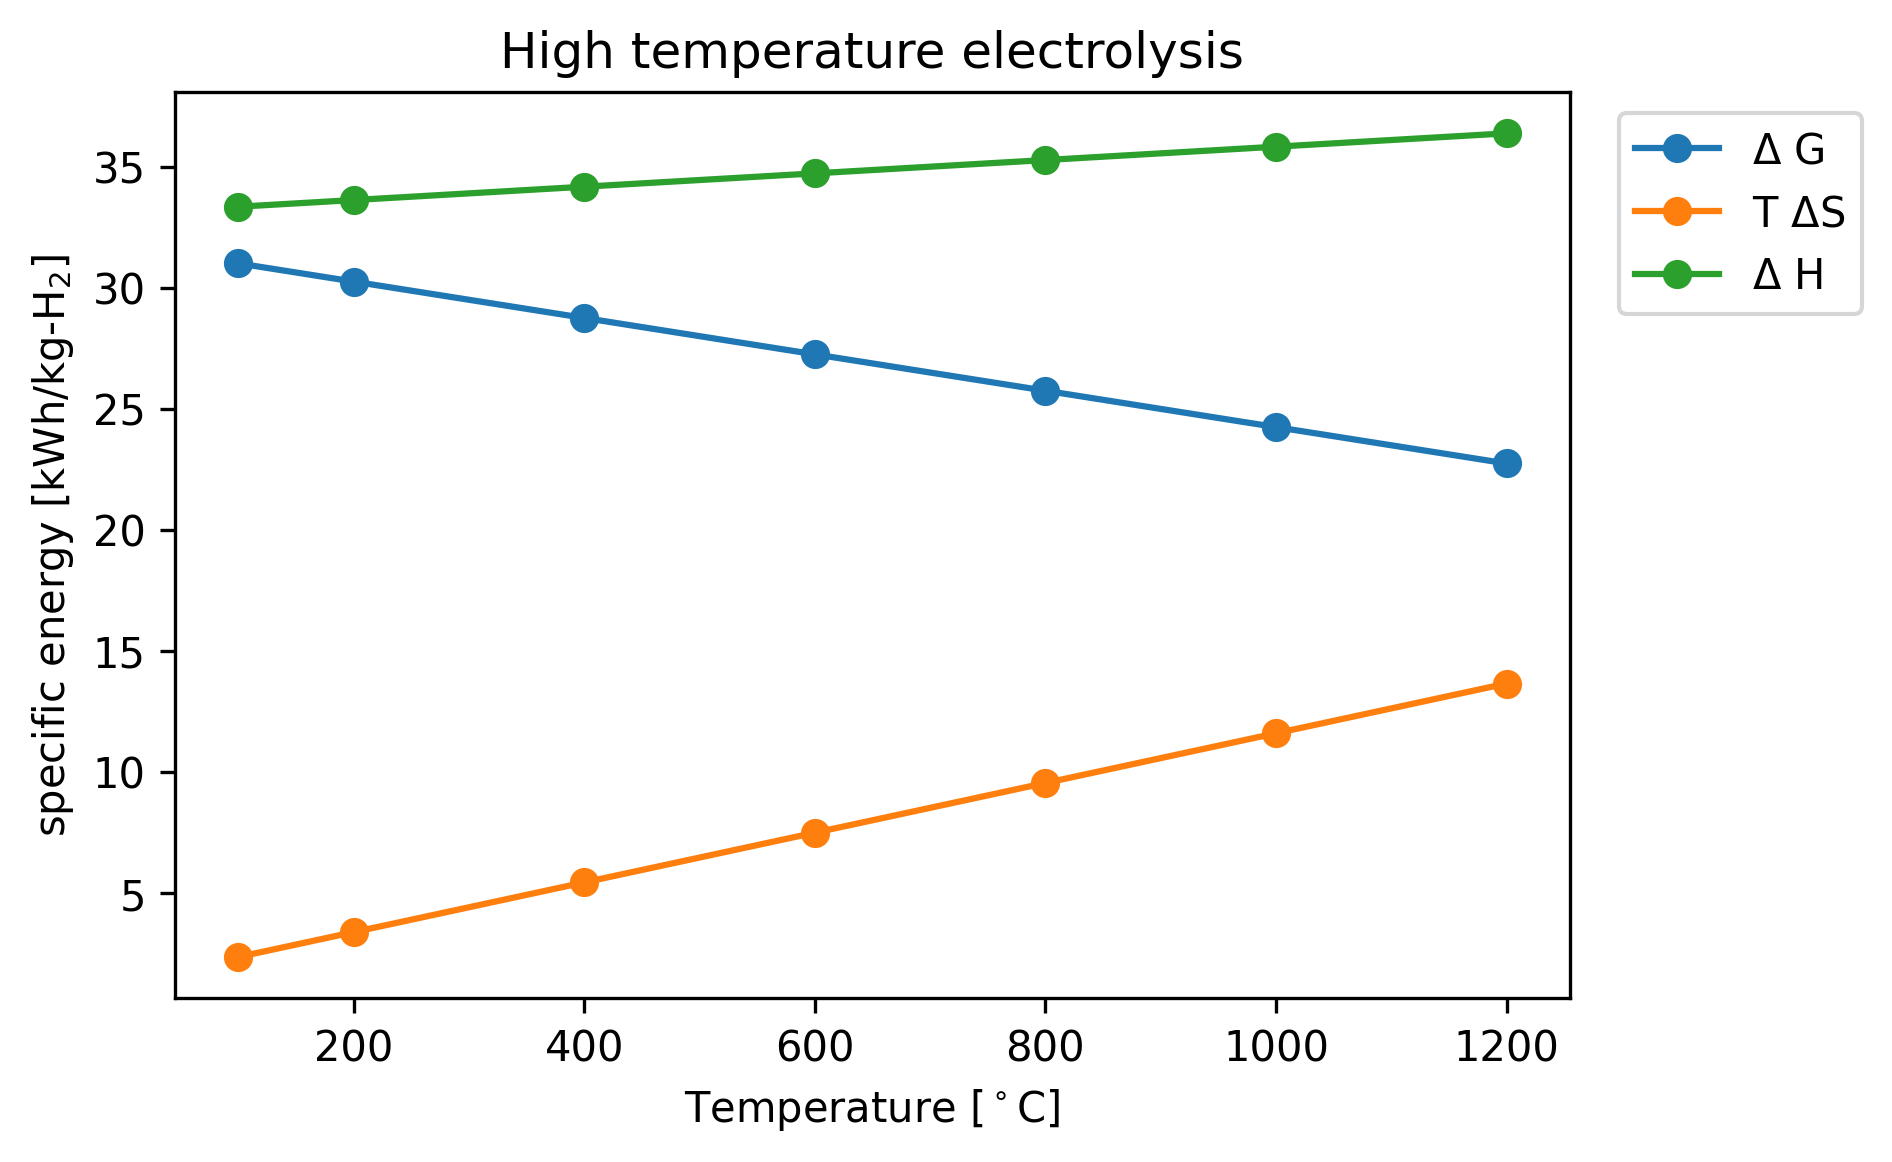
\includegraphics[width=0.8\linewidth]{figures/hte-energy.png}
	\hfill
	\caption{Energy required by an ideal \gls{HTE} process. Data from \cite{yildiz_efficiency_2006}.}
	\label{fig:electro1}
\end{figure}

\subsection{Sulfur-Iodine Thermo-chemical cycle}

The Sulfur-Iodine cycle consists of the three chemical reactions represented in Figure \ref{fig:sulfur1}.
The chemical reactions are:

\begin{align}
	& I_2 + SO_2 + 2H_2O \rightarrow 2HI + H_2SO_4 \\
	\label{eq:sulfur1}
	& H_2SO4 \rightarrow SO_2 + H_2O + 1/2O_2 \\
	\label{eq:sulfur2}
	& 2HI \rightarrow I_2 + H_2. \\
	\label{eq:sulfur3}
\end{align}

The whole process takes in water and high temperature heat, and releases hydrogen and oxygen.
The process does not use any electricity.
The process recycles all reagents and does not have any effluents \cite{yildiz_efficiency_2006}.

Figure \ref{fig:sulfur2} presents the specific energy requirements of the cycle $\Delta H$.
Equation \ref{eq:sulfur4} determines the thermal energy required by the hydrogen plant $P_{TH2}$.

\begin{align}
	P_{TH2} &= \dot{m}_{H2} \Delta H\\
	\label{eq:sulfur4}
	\intertext{where}
	P_{TH2} &= \mbox{total thermal energy} \\
	\dot{m}_{H2} &= \mbox{\gls{H2} production rate} \\
	\Delta H &= \mbox{specific energy} \\
\end{align}

Note the discrepancy between Figure \ref{fig:sulfur1} and Figure \ref{fig:sulfur2} of the high temperature required.
Other sources seem to disagree in that number too.
Our analysis considers the process viable only for temperatures above 800 $^{\circ}$C.

\begin{figure}[htbp!]
	\centering
	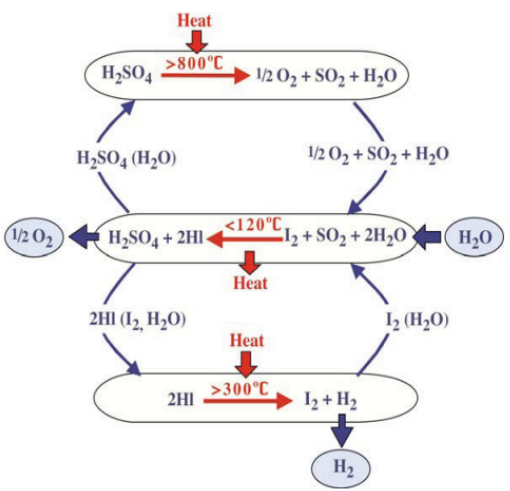
\includegraphics[width=0.7\linewidth]{figures/sulfur1.png}
	\hfill
	\caption{Diagram of the Sulfur-Iodine Thermochemical process. Image reproduced from \cite{benjamin_russ_sulfur_2009}.}
	\label{fig:sulfur1}
\end{figure}

\begin{figure}[htbp!]
	\centering
	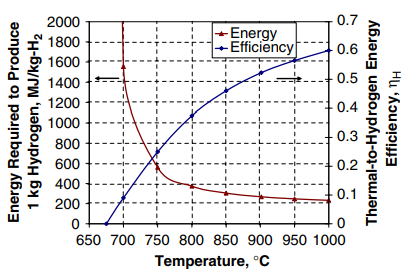
\includegraphics[width=0.7\linewidth]{figures/si-energy.png}
	\hfill
	\caption{Energy required by the Sulfur-Iodine Cycle. Image reproduced from \cite{yildiz_efficiency_2006}.}
	\label{fig:sulfur2}
\end{figure}

\section{Microreactors and \glspl{SMR}}
\label{sec:reactors}

% shared characteristics of SMRs and Micro-R
The typical \gls{UIUC}'s grid demand is smaller than 80 MW \cite{dotson_optimal_2020}.
Accordingly, we consider reactors of small capacities, such as microreactors and \glspl{SMR}.

% Microreactor features
A microreactor has three main features: it is factory fabricated, transportable, and self-regulating.
All of the components are fully assembled in a factory and shipped out to the generation site, reducing capital costs and enabling rapid deployment.
Small designs make it easy for vendors to ship the entire reactor by truck, shipping vessel, or railcar.
Simplified design concepts enhance self-regulating capabilities and eliminate the need for many specialized operators and maintenance staff.
Moreover, they utilize passive safety systems that prevent overheating or meltdown.
These main features make the technology appealing for a wide range of applications, such as deployment in remote residential locations and military bases \cite{us-doe_ultimate_2019}.

% SMR features
\glspl{SMR} require limited on-site preparation as their components are factory fabricated, reducing up-front capital costs and expediting start-up times.
This reactor concept allows for black starts and islanding operation mode.
They can start up from a completely de-energized state without receiving power from the grid.
They can also operate connected to the grid or independently.
Moreover, they minimize electrical parts and use passive cooling features to safely shutdown.
Other benefits include underground construction, which makes reactors less vulnerable to extreme weather and physical attacks \cite{us-doe_ultimate_2019}.

These reactor concepts share several features.
The \gls{DOE} defines a microreactor as a reactor that generates from 1 to 20 MW$_{th}$ \cite{us-doe_ultimate_2019}.
The \gls{IAEA} describes a \gls{SMR} as a reactor whose power is under 300 MWe.
However, it adds another definition.
It defines a very small modular reactor as a reactor that produces less than 15 MWe \cite{world_nuclear_association_small_2020}.
There is clearly an overlap in the definitions, but we will not discuss it.
We will consider reactors of less than 100 MW$_{th}$ regardless of their classification.

\section{Methodology}
\label{sec:metho}

In this analysis, the energy source (both electric and thermal) is a nuclear reactor with co-generation capabilities.
The nuclear reactor supplies the grid with electricity ($P_E$) while providing a hydrogen plant with electricity ($P_{EH2}$) and thermal energy ($P_{TH2}$), Figure \ref{fig:cogen}.
$\beta$ and $\gamma$ determine the distribution of the reactor thermal power $P_{th}$ into $P_E$, $P_{EH2}$, and $P_{TH2}$, see Equations \ref{eq:cogen1} to \ref{eq:cogen6}.

\begin{figure}[htbp!]
	\centering
	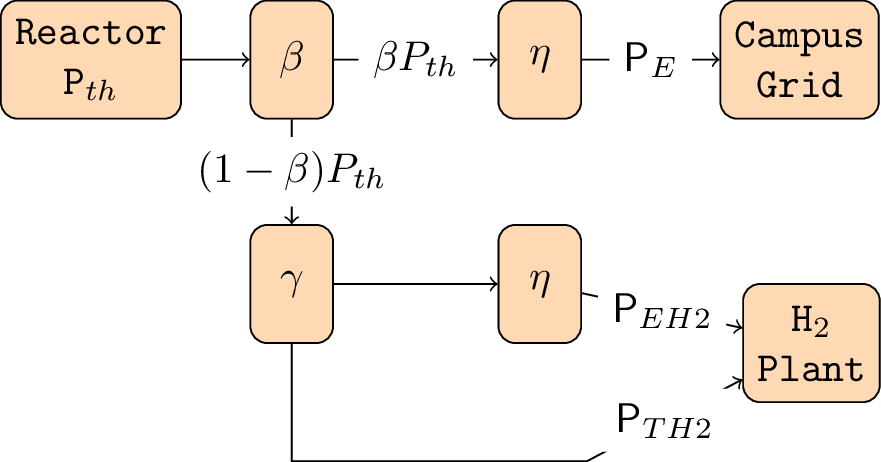
\includegraphics[height=3.6cm]{figures/hte-figure0.png}
	\hfill
	\caption{Diagram of a reactor coupled to hydrogen plant.}
	\label{fig:cogen}
\end{figure}

\begin{equation}
\begin{split}
	P_{E} &= \eta \beta P_{th}
	\\
	P_{EH2} &= \eta \gamma (1-\beta) P_{th}
	\\
	P_{TH2} &= (1-\gamma) (1-\beta) P_{th}
	\\
	\gamma &= \frac{P_{EH2} / \eta}{P_{EH2} / \eta + P_{TH2}}
	\\
	\beta &= \frac{P_{E} / \eta}{P_{E} / \eta + P_{TH2}/(1-\gamma)}.
\end{split}
\label{eq:hydro}
\end{equation}

\begin{align}
	P_{E} &= \eta \beta P_{th} \\
	\label{eq:cogen1}
	P_{EH2} &= \eta \gamma (1-\beta) P_{th}\\
	\label{eq:cogen2}
	P_{TH2} &= (1-\gamma) (1-\beta) P_{th}\\
	\label{eq:cogen3}
	\intertext{where}
    \eta &= \mbox{thermal-to-electric conversion efficiency} \\
	\label{eq:cogen4}
	\beta &= \frac{P_{E} / \eta}{P_{E} / \eta + P_{TH2}/(1-\gamma)}\\
	\label{eq:cogen5}
	\gamma &= \frac{P_{EH2} / \eta}{P_{EH2} / \eta + P_{TH2}}\\
	\label{eq:cogen6}
\end{align}

If $\beta = 1$, the reactor only supplies the grid with electricity $P_E$ and the hydrogen plant does not produce \gls{H2}.
If $\beta = 0$, the reactor only supplies the hydrogen plant and now electricity goes into the grid.
Table \ref{tab:cogen1} summarizes the values that $\gamma$ takes for the different methods.

\begin{table}[htbp!]
    \centering
    \begin{tabular}{|lccc|}
        \hline
        Method    & $\gamma$         & $P_{EH2}$ & $P_{TH2}$ \\ \hline
        \gls{LTE} & 1                & $\ne$ 0   & 0         \\
        \gls{HTE} & $0 < \gamma < 1$ & $\ne$ 0   & $\ne$ 0   \\
        \gls{SI}  & 0                & 0         & $\ne$ 0   \\ \hline
    \end{tabular}
    \caption{Energy requirements of the different methods.}
    \label{tab:cogen1}
\end{table}

\section{Results}
\label{sec:Results}

This section holds the results of the different analysis.

\subsection{Transportation}

Figure \ref{fig:fuel} displays the fuel consumed per day by \gls{MTD} and \gls{UIUC} fleet.
Using the values shown in Table \ref{tab:equiv}, we calculate the hydrogen requirement for MTD and UIUC fleets, Figure \ref{fig:hydro-fleet}.
Table \ref{tab:hydro-fleet} summarizes the most important results.

	\begin{figure}[htbp!]
		\centering
		\begin{subfigure}[t]{0.4\textwidth}
			\centering
			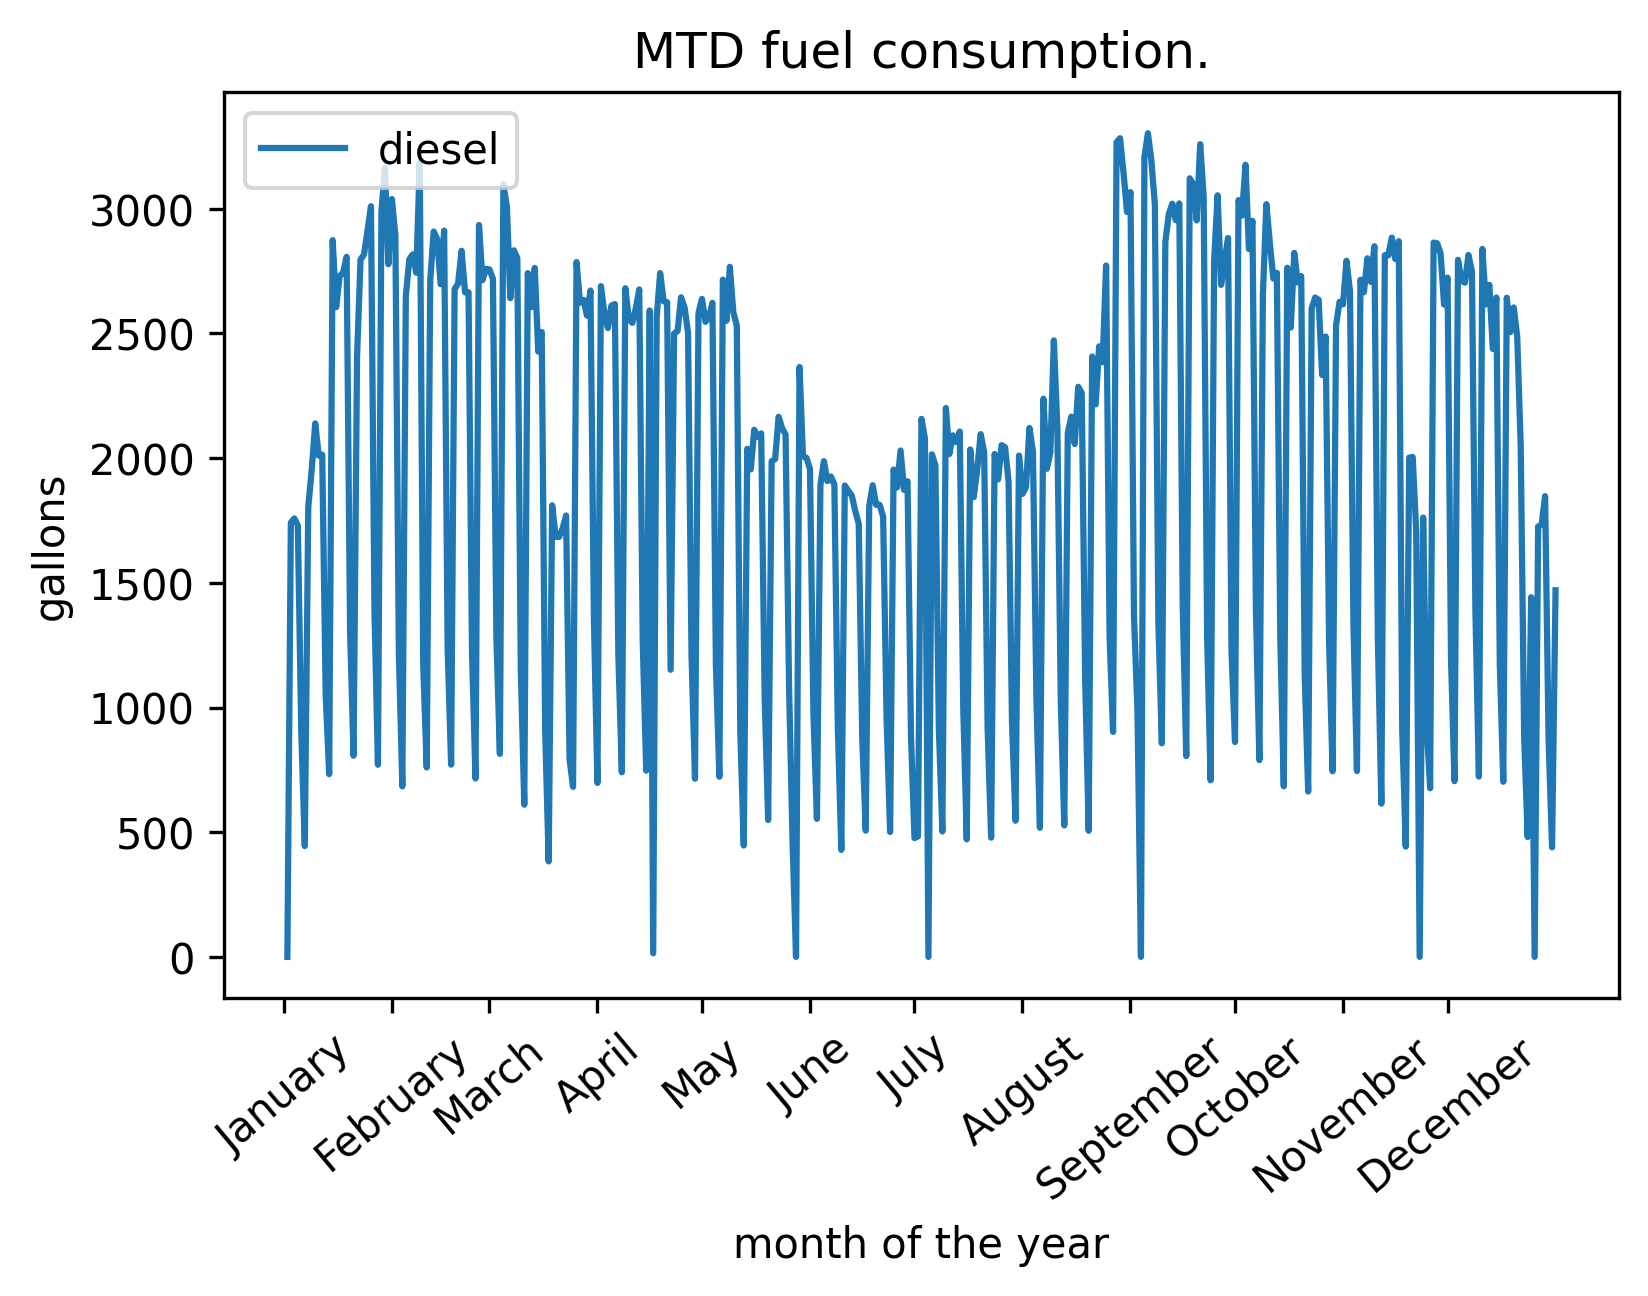
\includegraphics[width=\linewidth]{figures/mtd2}
			\caption{\gls{MTD} fleet. Data goes from July 1, 2018, until June 30, 2019 \cite{mtd_irecords_2019}.}
		\end{subfigure}
		\begin{subfigure}[t]{0.4\textwidth}
			\centering
			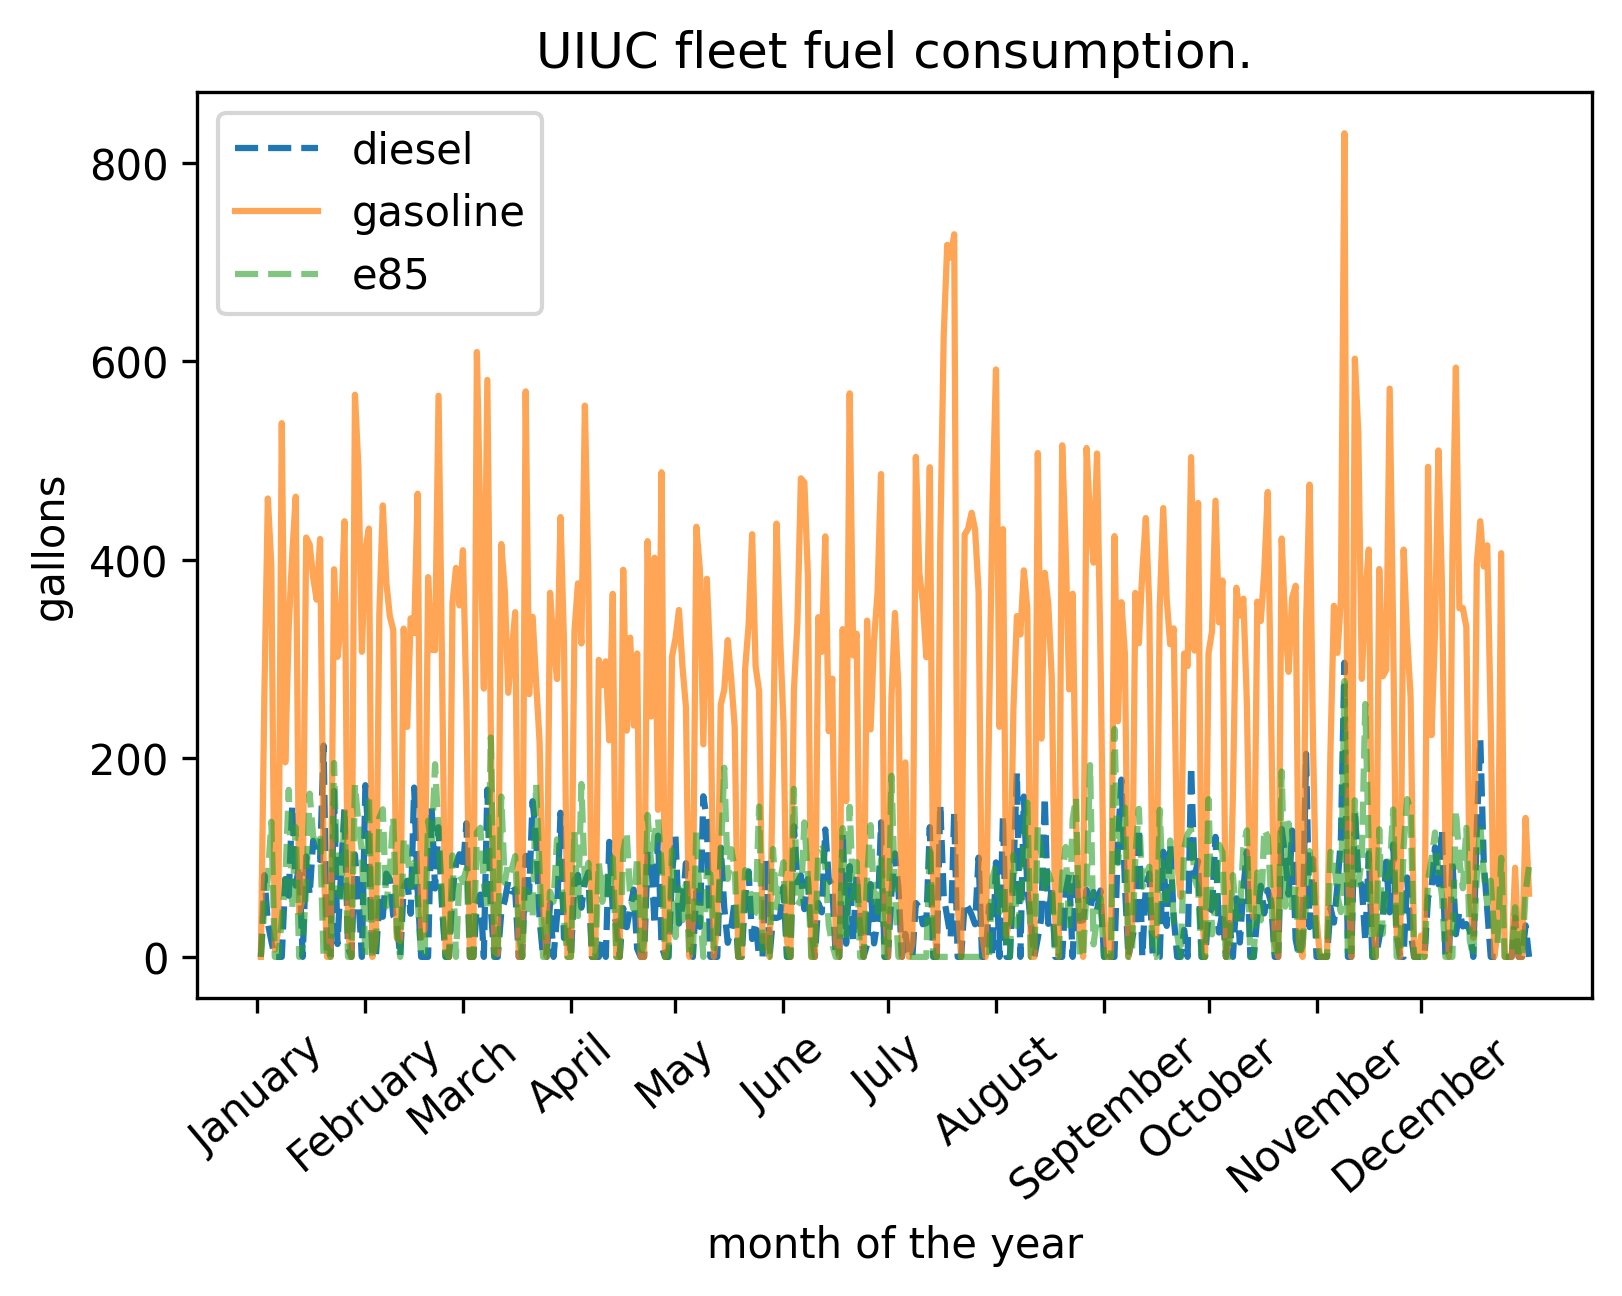
\includegraphics[width=\linewidth]{figures/uiuc}
			\caption{\gls{UIUC} fleet. Data goes from January 1, 2019, until December 31, 2019 \cite{uiuc_personnal_communication}.}
		\end{subfigure}
		\hfill
		\caption{Fuel consumption.}
		\label{fig:fuel}
	\end{figure}

	\begin{table}[htbp!]
	\centering
	\caption{Hydrogen mass necessary to replace a gallon of fuel \cite{doe_office_of_energy_efficiency_and_renewable_energy_hydrogen_2020} \cite{alternative_fuels_data_center_fuel_2014}.}
	\begin{tabular}{|l|c|}
	    \hline
	 	                 & Hydrogen Mass [kg] \\ \hline
	 	Gasoline         & 1                  \\
	 	Diesel           & 1.13               \\
	 	E85              & 0.78               \\ \hline
	\end{tabular}
	\label{tab:equiv}
	\end{table}

	\begin{figure}[htbp!]
	    \centering
		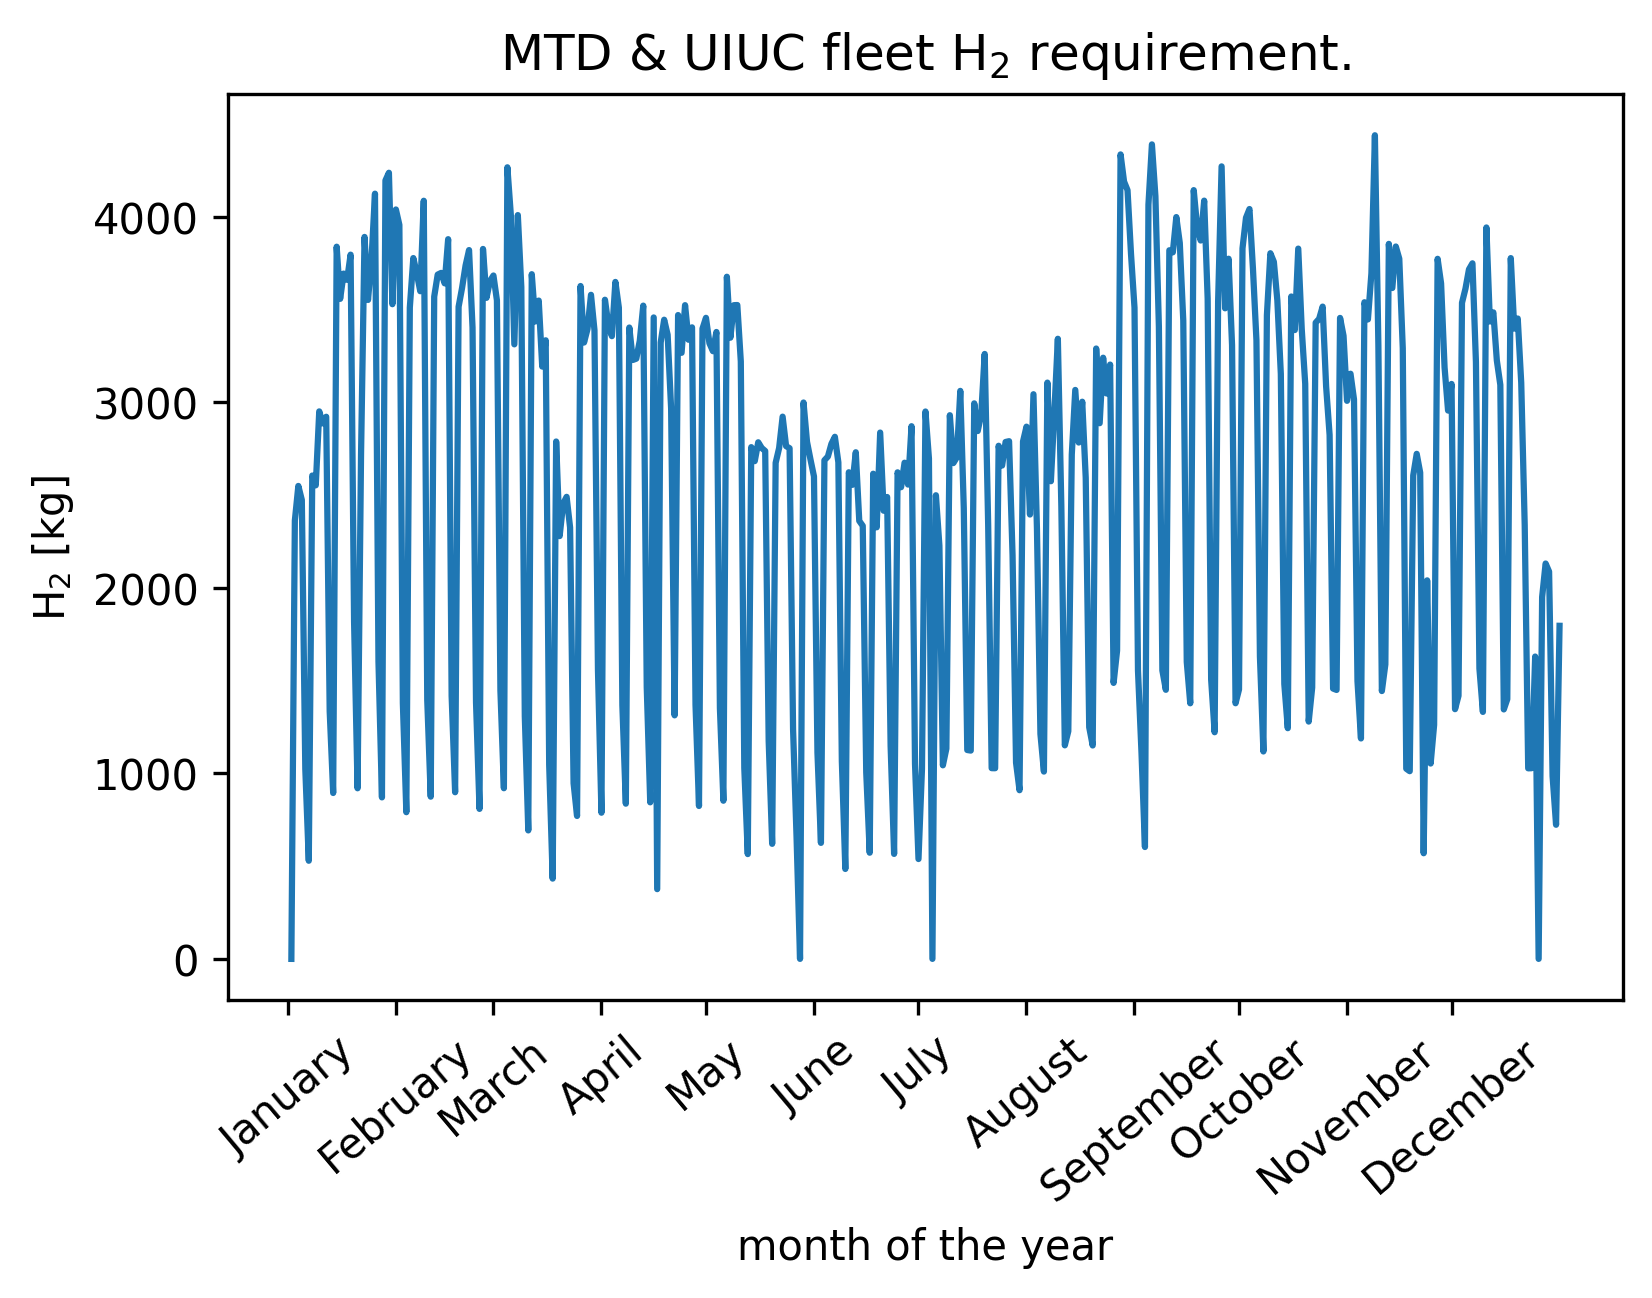
\includegraphics[height=6.0cm]{figures/hydro-fleet}
		\hfill
		\caption{Hydrogen requirement for MTD and UIUC fleets.}
		\label{fig:hydro-fleet}
	\end{figure}

	\begin{table}[htbp!]
		\centering
	    \caption{Hydrogen requirements.}
		\begin{tabular}{|l|c|}
		\hline
		Total [tonnes/year]     & 943    \\
		Average [kg/day] 	    & 2584   \\
		Average [kg/h] 		    & 108    \\
		Maximum in one day [kg] & 4440   \\ \hline
        \end{tabular}
        \label{tab:hydro-fleet}
	\end{table}

Using Table \ref{tab:co2-eq}, we calculate the \gls{CO2} savings caused by replacing all the fossil fuels by \gls{H2}.
Table \ref{tab:co2} displays the \gls{CO2} savings for both fleets.

	\begin{table}[htbp!]
		\centering
	    \caption{\gls{CO2} savings in lbs per gallon of fuel burned \cite{energy_information_administration_how_2014}.}
		\begin{tabular}{|l|c|}
		\hline
		              & \gls{CO2} produced [lbs/gallon] \\ \hline
		Gasoline      & 19.64           \\
		Diesel        & 22.38           \\
		E85           & 13.76           \\ \hline
        \end{tabular}
        \label{tab:co2-eq}
	\end{table}

	\begin{table}[htbp!]
		\centering
	    \caption{\gls{CO2} yearly savings.}
		\begin{tabular}{|l|c|}
		\hline
		            & \gls{CO2} mass [tonnes] \\ \hline
		MTD      	& 7306           \\
		UIUC        & 1143           \\
		Total       & 8449           \\ \hline
        \end{tabular}
        \label{tab:co2}
	\end{table}

% I stopped here

	\begin{table}[htbp!]
		\centering
	    \caption{Microreactor designs.}
		\begin{tabular}{|lcc|}
		\hline
		Reactor                                      & P[MW$_{th}$] & T$_o$[$^\circ$C] \\ \hline
		MMR \cite{usnc_mmr_2019}  		             & 15           & 640              \\
		eVinci \cite{hernandez_micro_2019}           & 5            & 650              \\
		ST-OTTO \cite{harlan_x-energy_2018}          & 30           & 750              \\
		U-battery \cite{ding_design_2011}            & 10           & 750              \\
		Starcore \cite{star_core_nuclear_star_2015}  & 36           & 850              \\ \hline
        \end{tabular}
        \label{tab:hydro-micro}
	\end{table}

	% need to re-do this figure: SI only feasible for T > 800
	\begin{figure}[htbp!]
	    \centering
		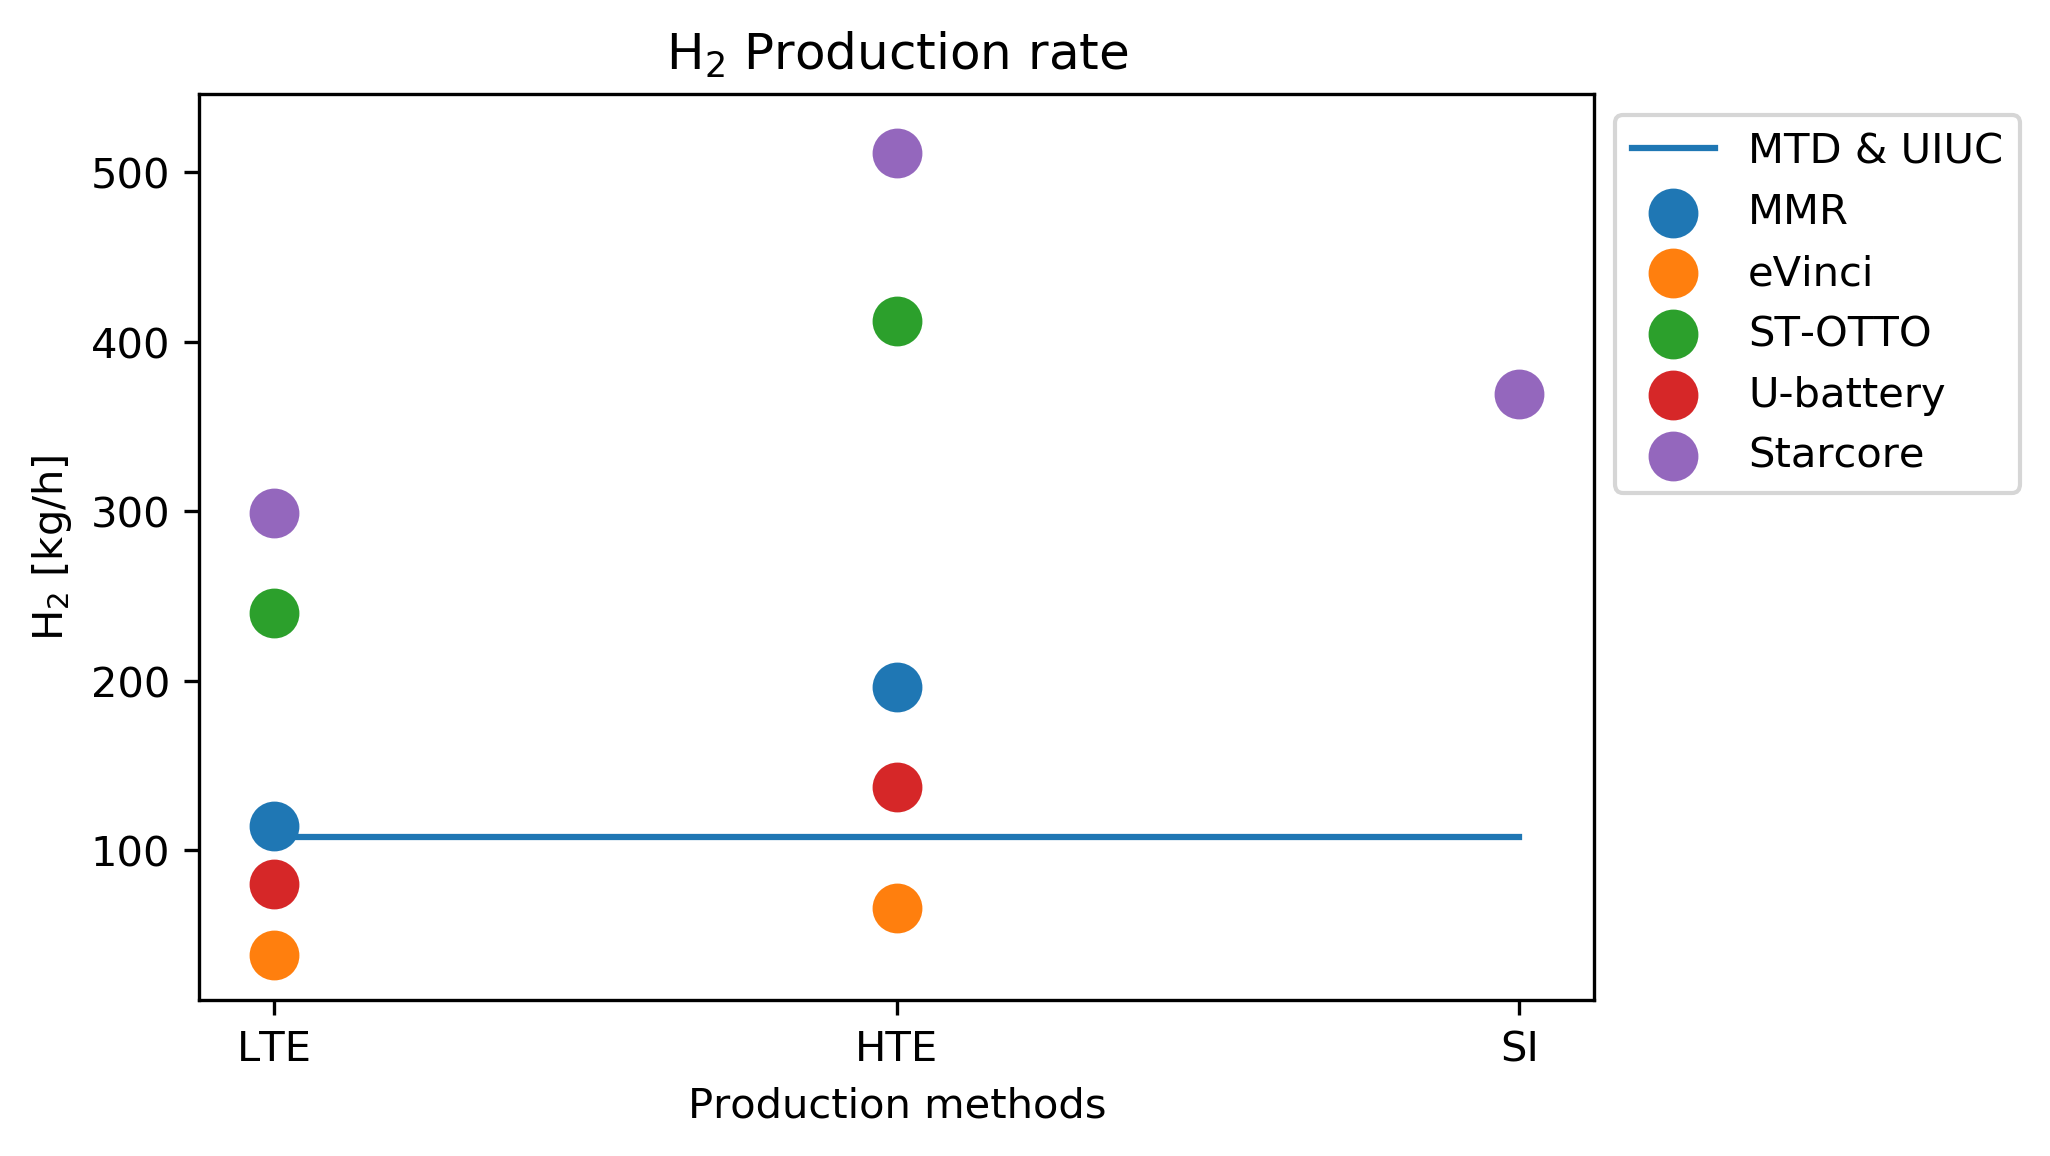
\includegraphics[height=4.3cm]{figures/reactors-by-hour1}
		\hfill
		\caption{Hydrogen production rate by the different microreactor designs.}
		\label{fig:hydro-micro}
	\end{figure}

\subsection{Electricity Generation}

% This last step enables us to decrease the need for dispatchable sources.

	\begin{figure}[htbp!]
		\centering
		\begin{subfigure}[t]{0.38\textwidth}
			\centering
			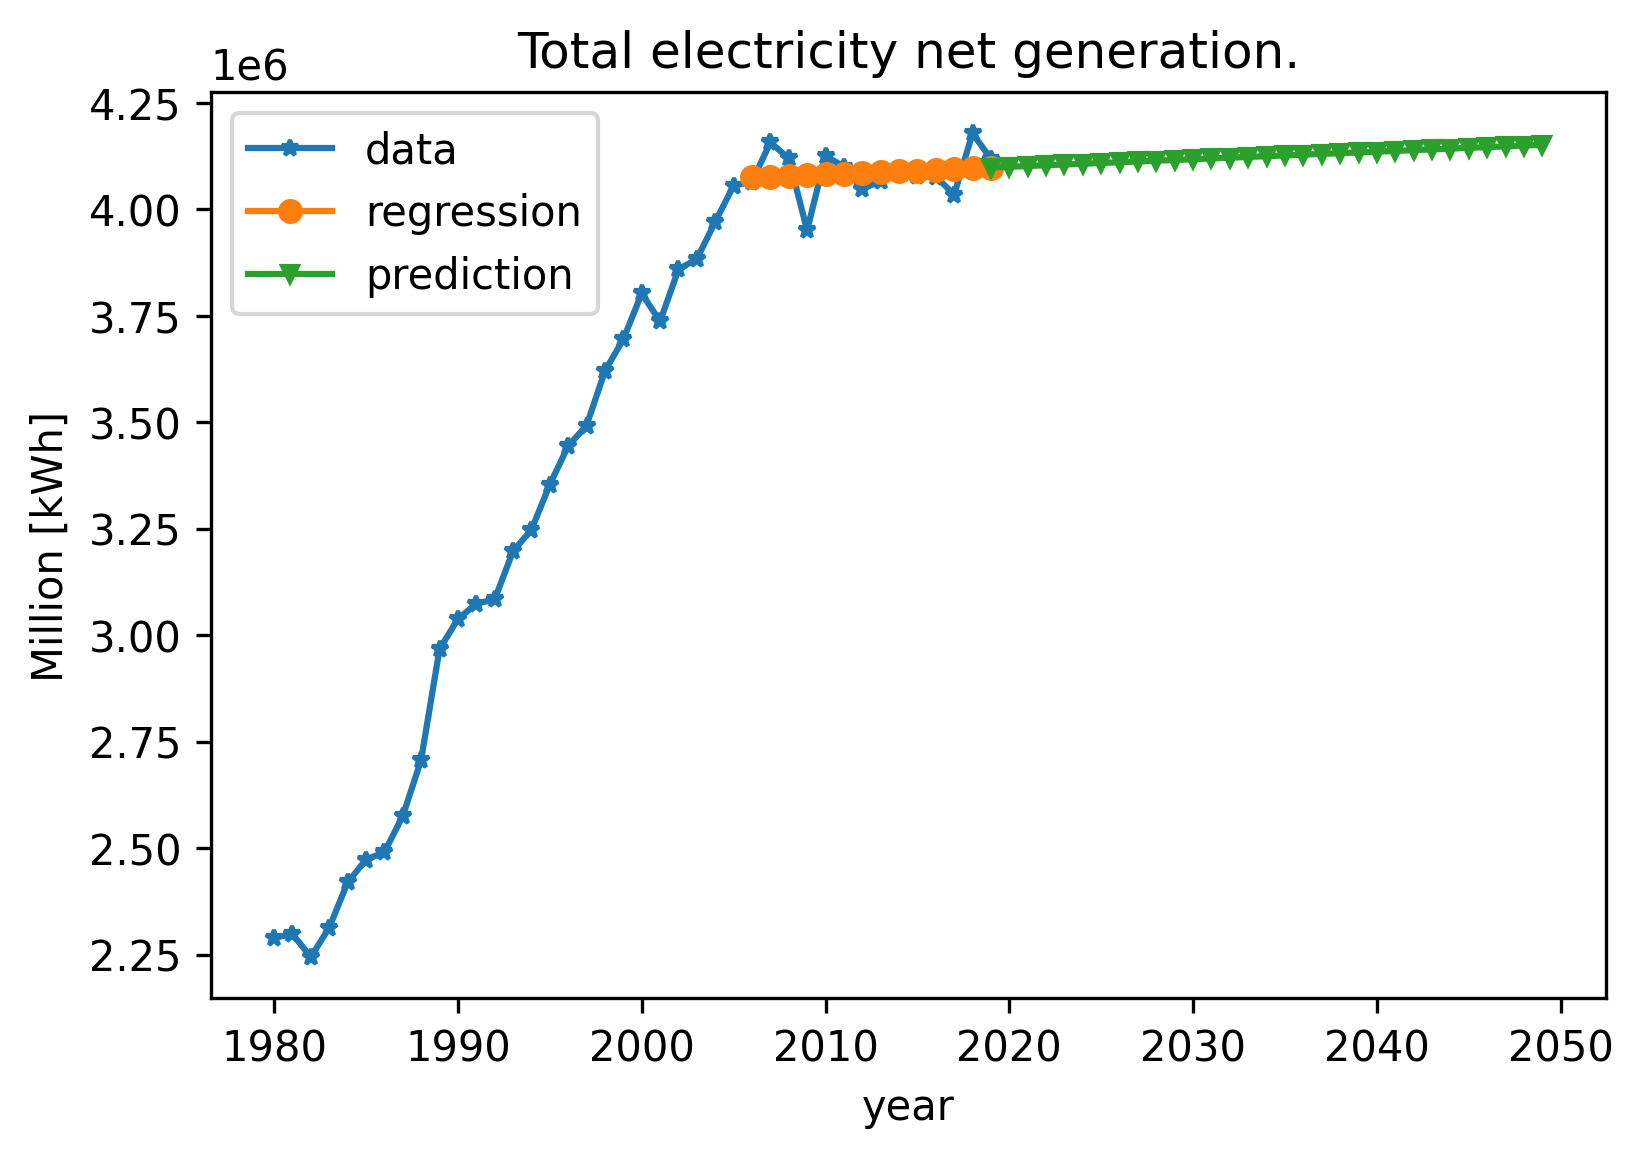
\includegraphics[width=\linewidth]{figures/us-prediction1}
			\caption{Total electricity generation.}
		\end{subfigure}
		\begin{subfigure}[t]{0.40\textwidth}
			\centering
			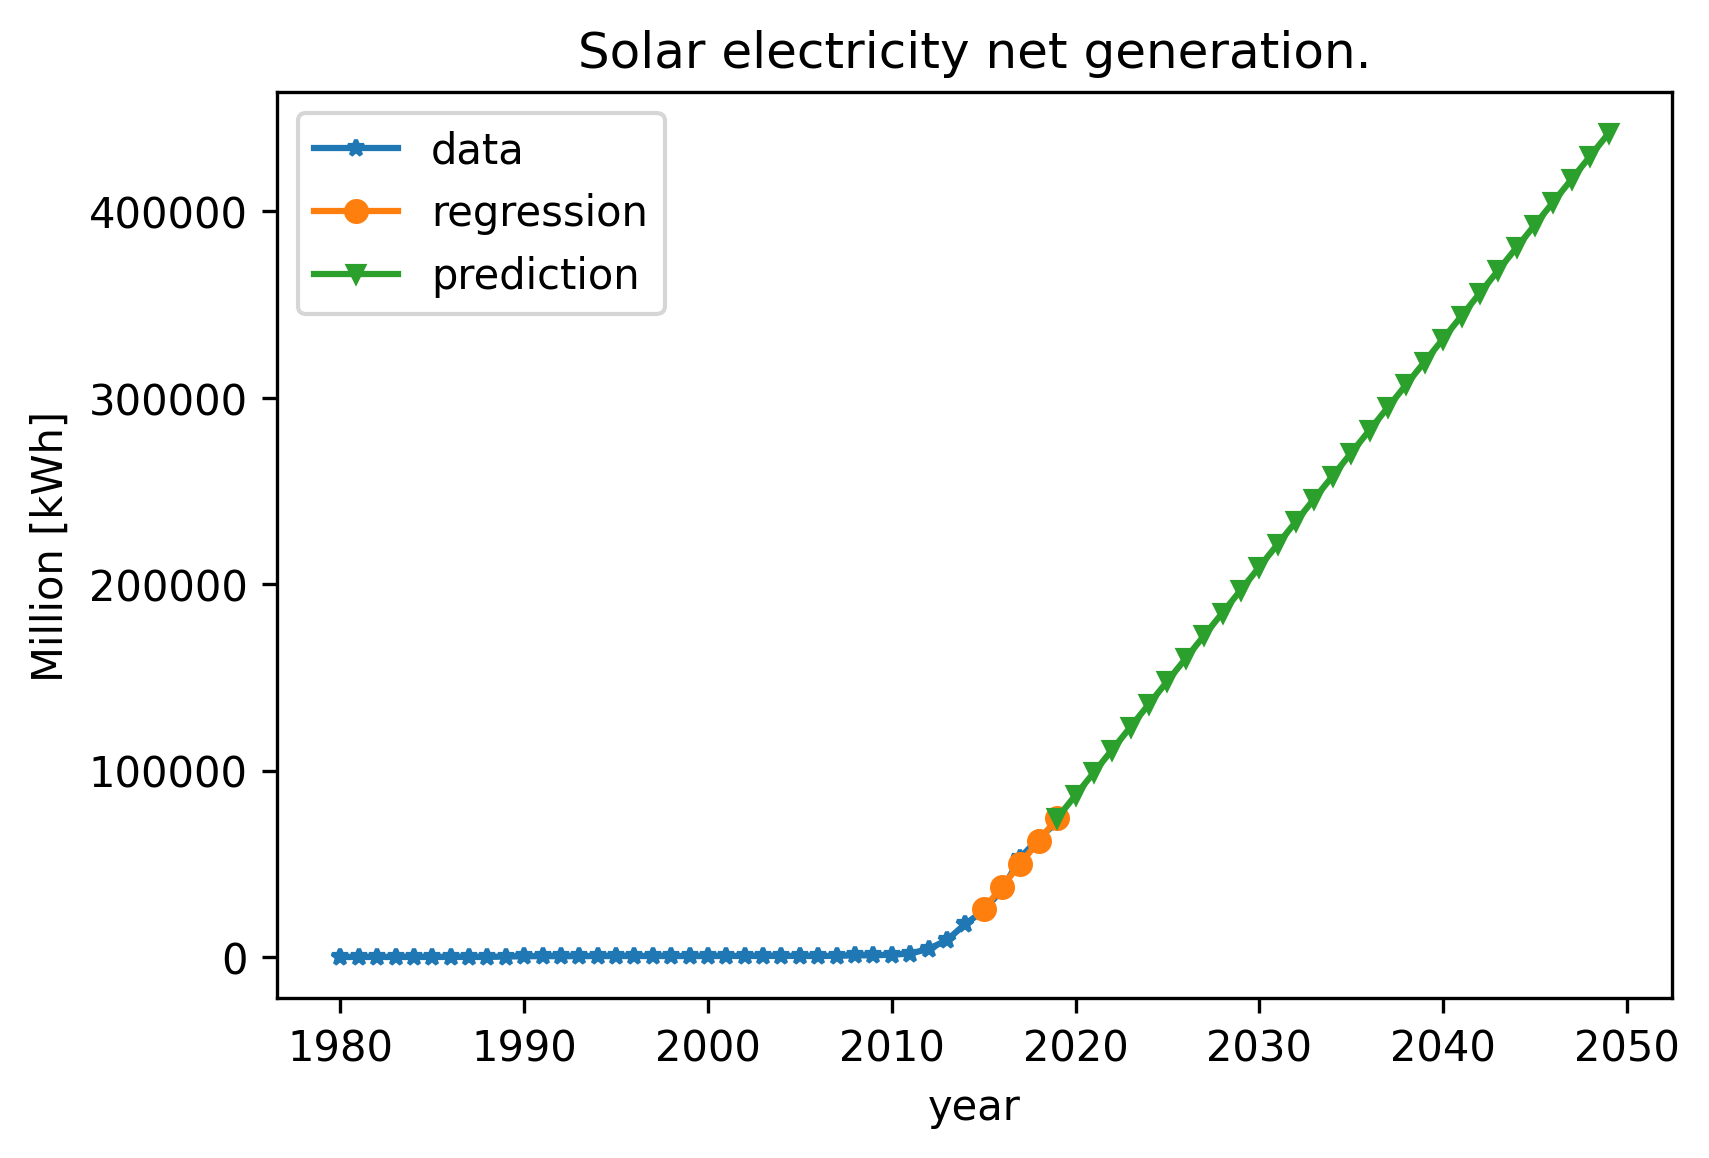
\includegraphics[width=\linewidth]{figures/us-prediction2}
			\caption{Solar electricity generation.}
		\end{subfigure}
		\hfill
		\caption{Prediction of the electricity generation in the \gls{US} for 2050. Data from \cite{us_energy_information_administration_electric_2020}.}
		\label{fig:prediction}
	\end{figure}

	\begin{figure}[htbp!]
	    \centering
		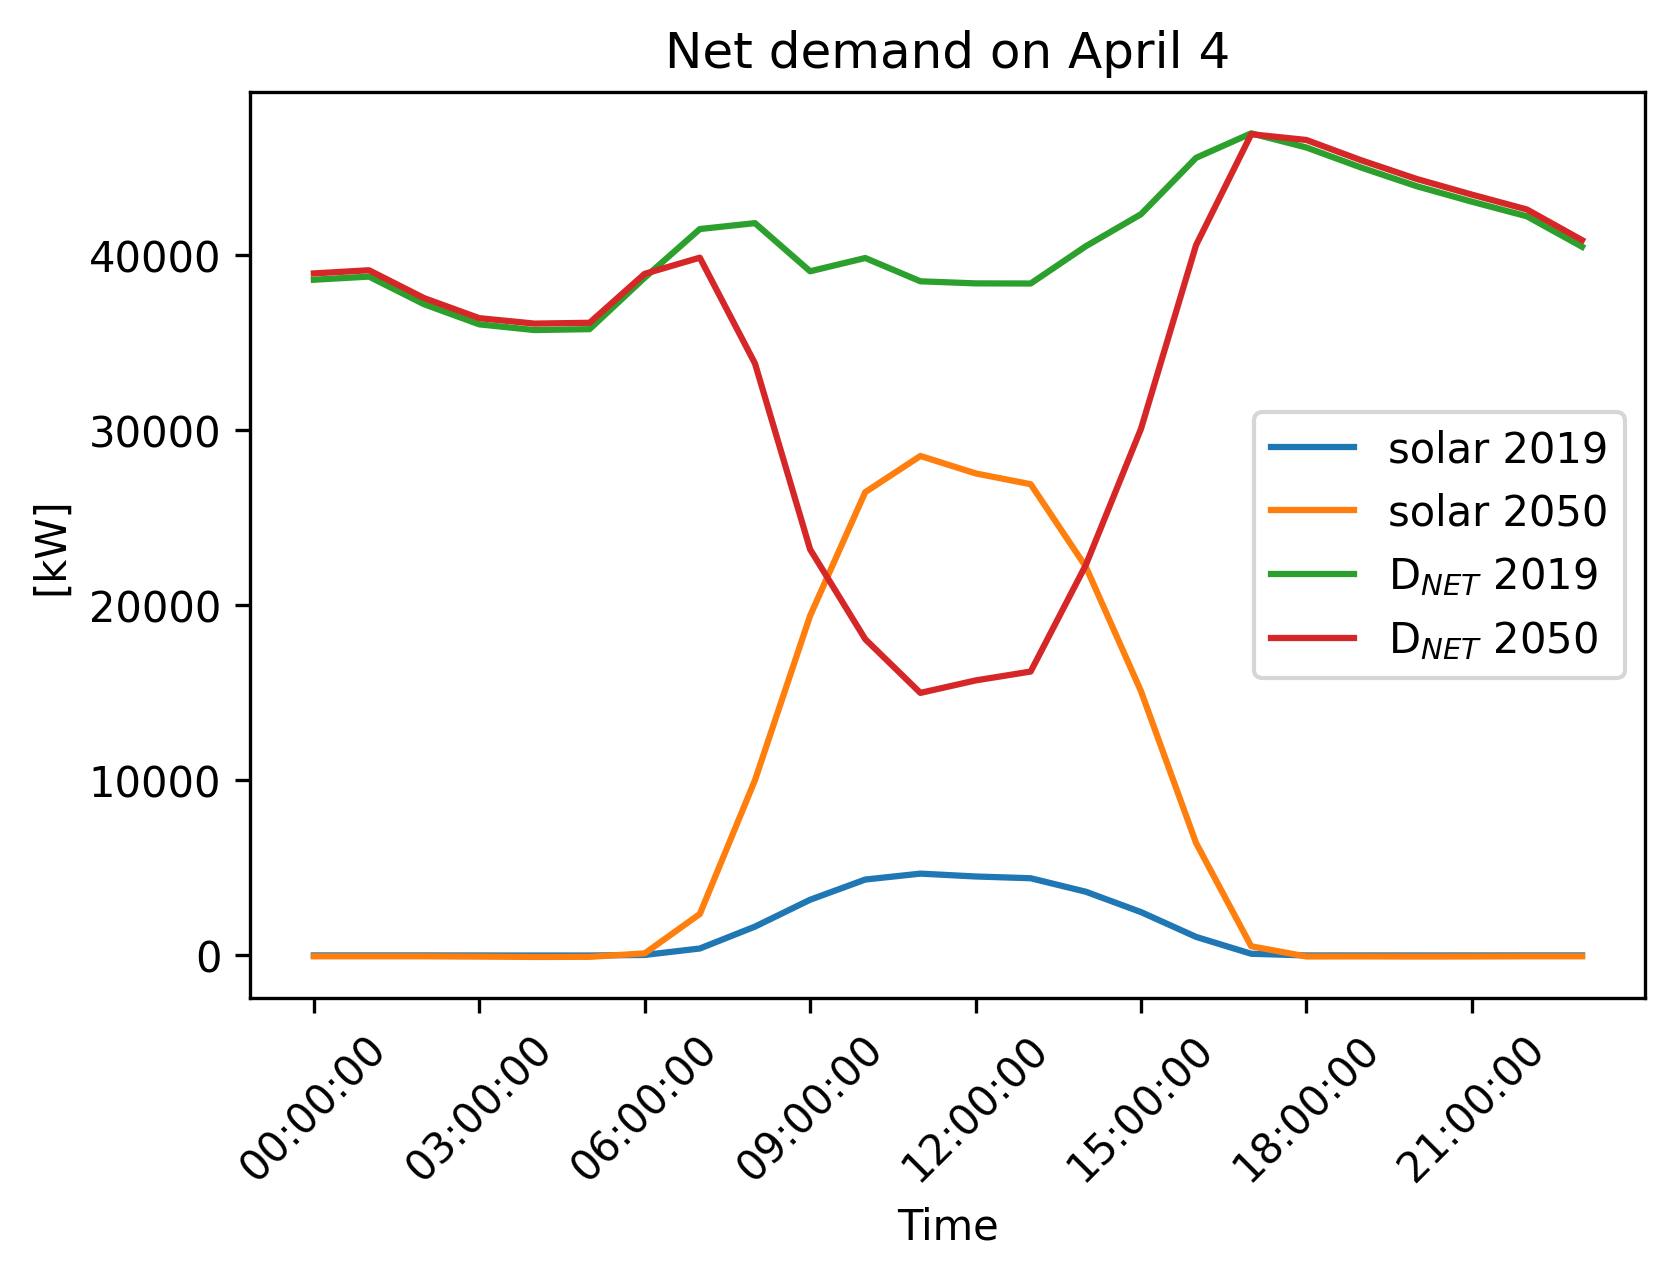
\includegraphics[height=4.3cm]{figures/uiuc-duck}
		\hfill
		\caption{Prediction of \gls{UIUC}'s net demand for 2050.}
		\label{fig:uiuc-duck1}
	\end{figure}

	\begin{figure}[htbp!]
	    \centering
		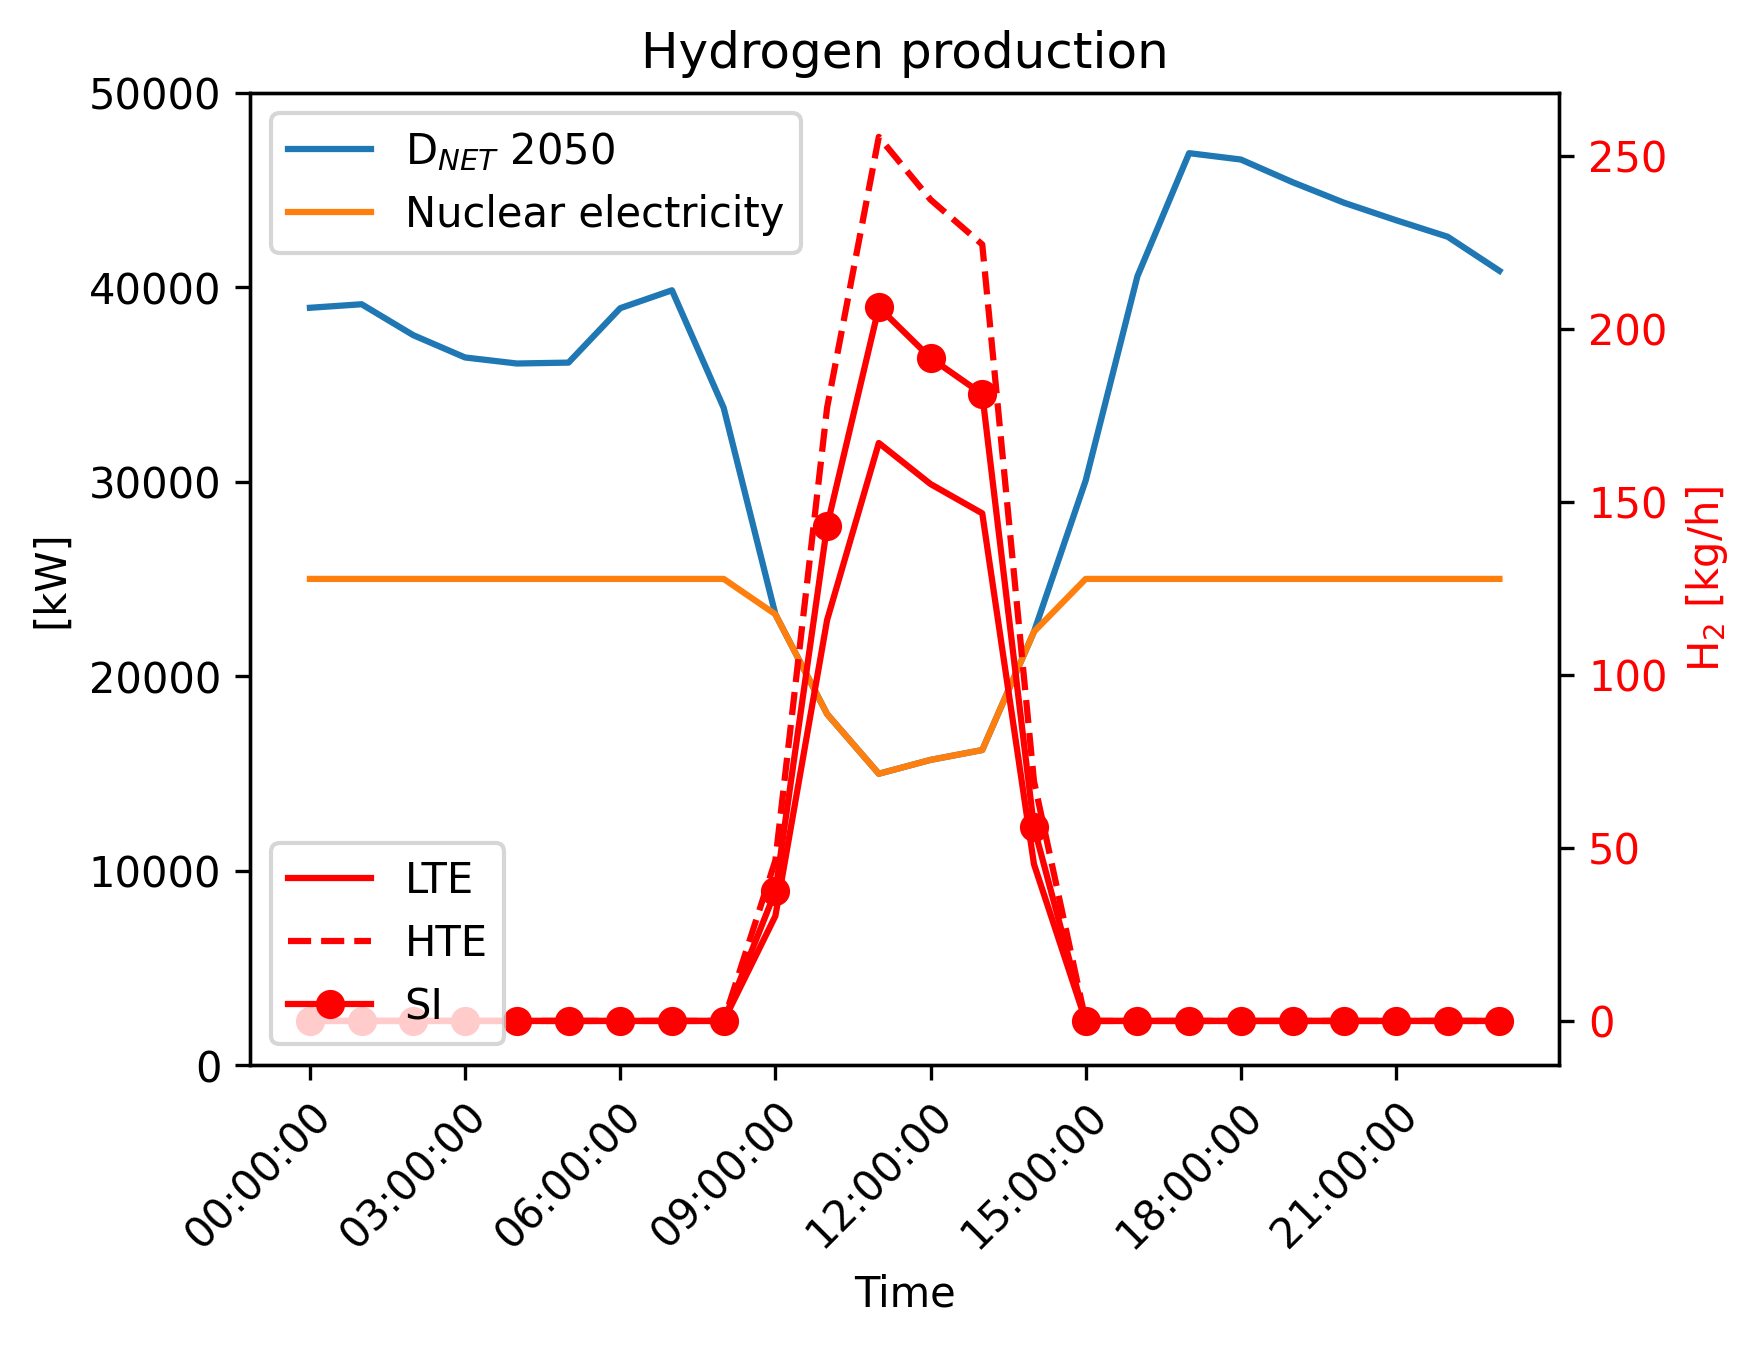
\includegraphics[height=4.3cm]{figures/uiuc-hydro2B}
		\hfill
		\caption{Hydrogen production with the excess of energy due to a net demand decrease.}
		\label{fig:uiuc-duck2}
	\end{figure}

	\begin{figure}[htbp!]
	    \centering
		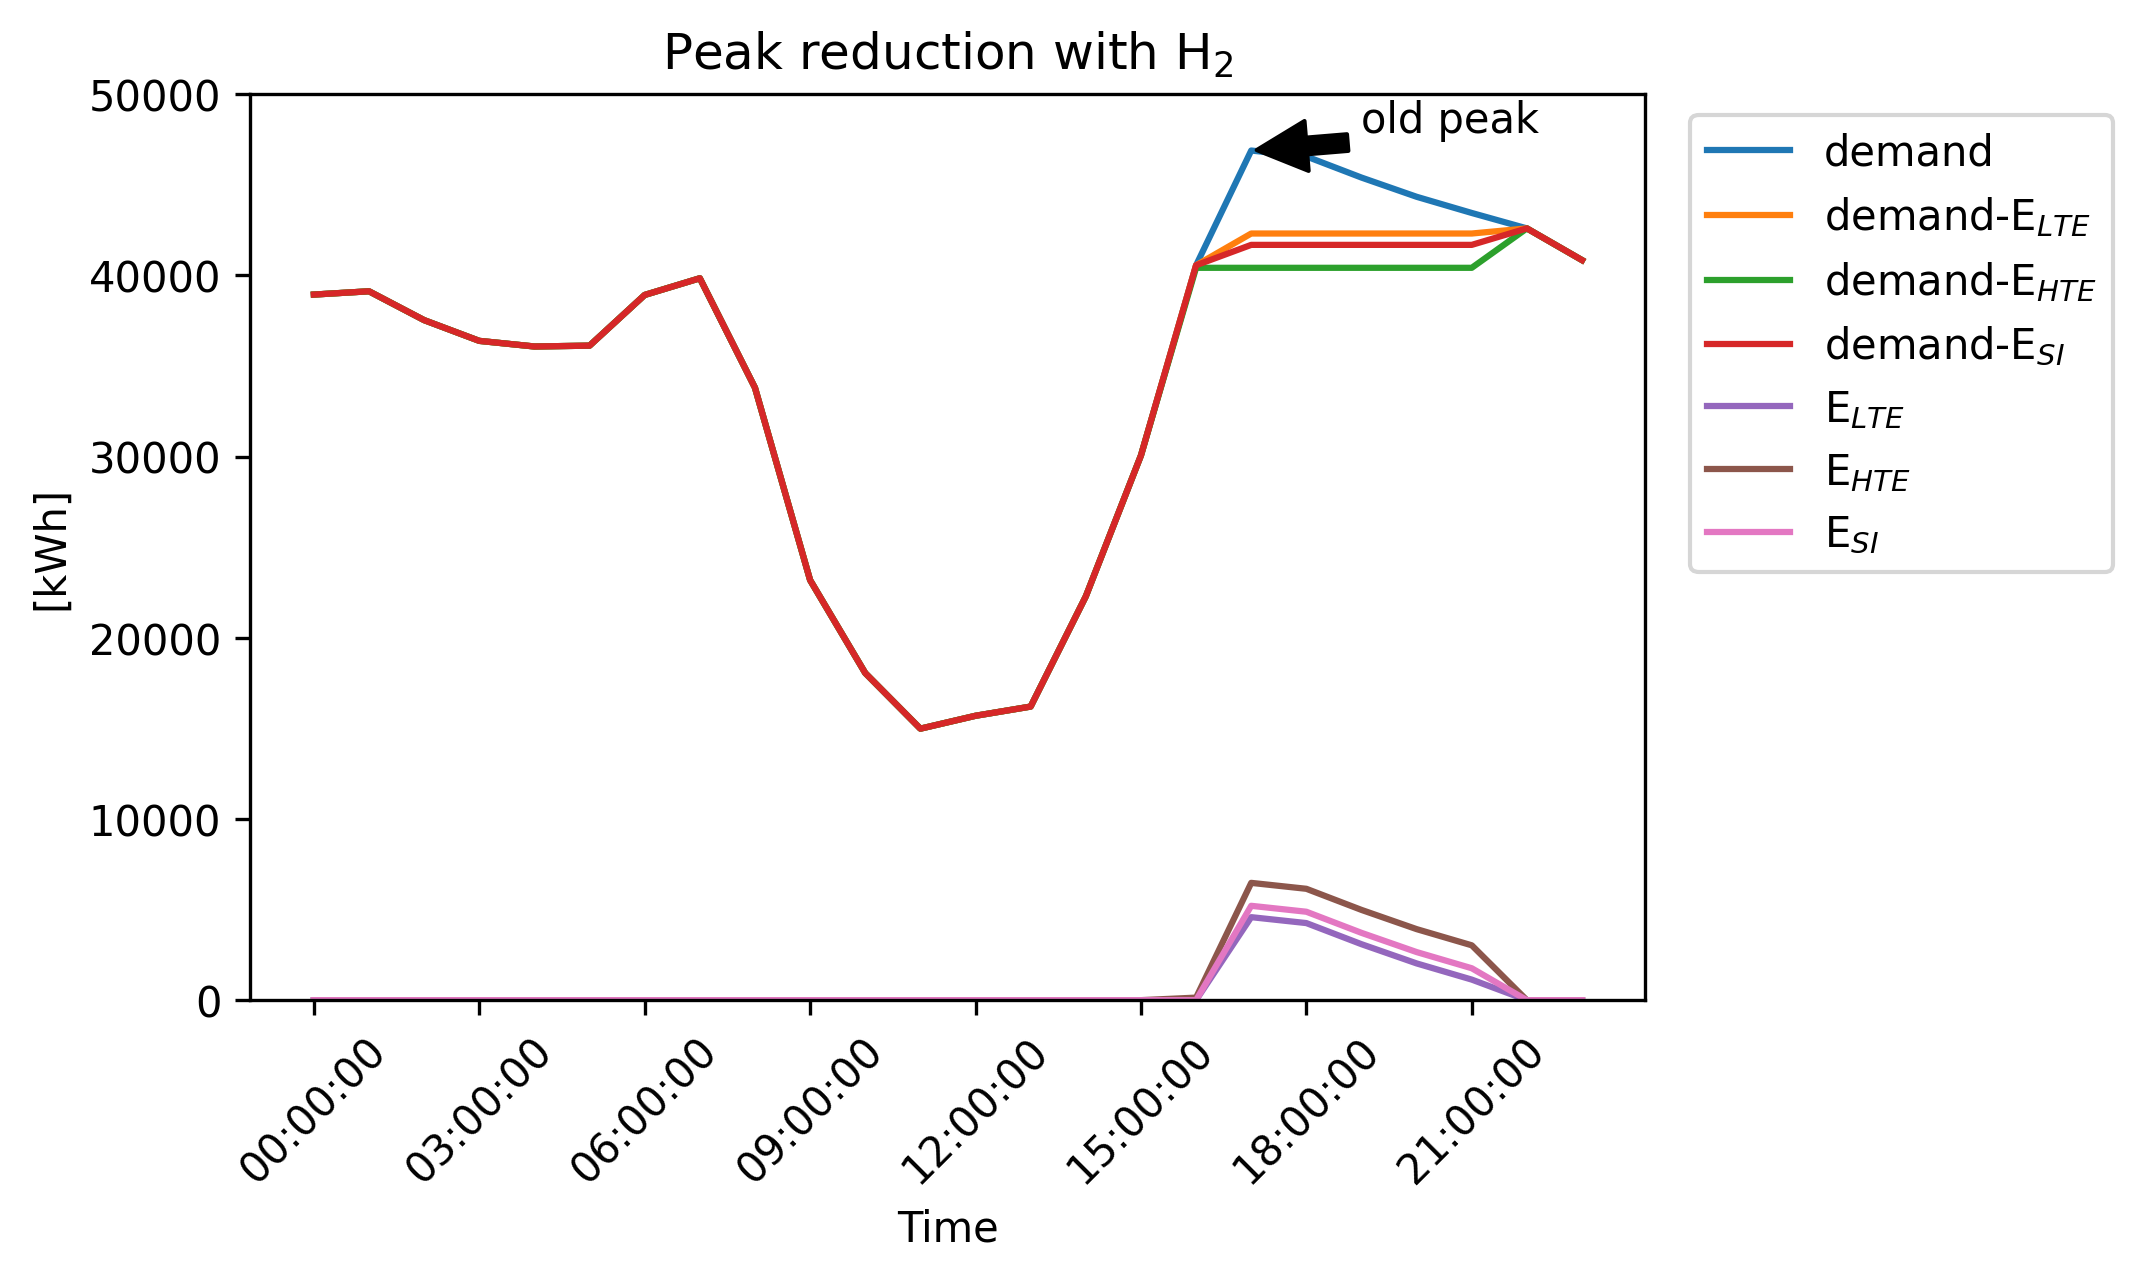
\includegraphics[height=4.3cm]{figures/uiuc-hydro3B}
		\hfill
		\caption{Peak reduction by using the produced H$_2$.}
		\label{fig:uiuc-duck3}
	\end{figure}




\section{Conclusions}

The University of Illinois is actively working to reduce GHG emissions on its campus. 

A few microreactor designs could produce enough hydrogen to meet MTD and UIUC fleet fuel demand.

Increased solar penetration worsens the duck curve.

Hydrogen introduces a way to store energy that reduces the reliance on dispatchable sources.

Nuclear energy and hydrogen production present an approach to mitigate the negative implications of the duck curve.


\pagebreak
\bibliographystyle{plain}
\bibliography{bibliography}

\end{document}

	% \begin{figure}[htbp!]
	% 	\centering
	% 	\begin{subfigure}[t]{0.4\textwidth}
	% 		\centering
	% 		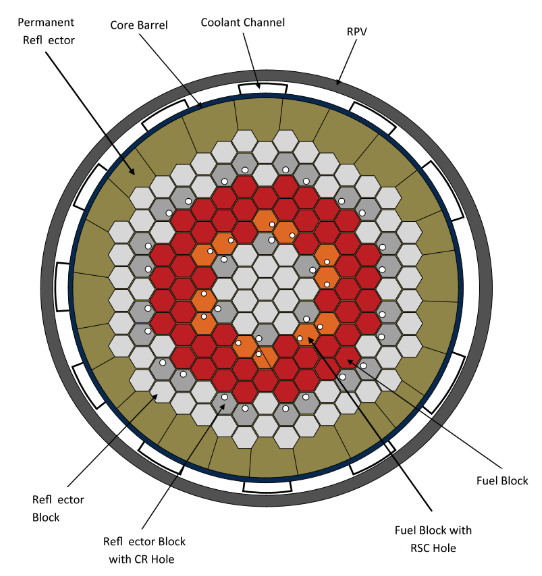
\includegraphics[width=\linewidth]{figures/radial-layout.png}
	% 		\caption{XY-plane.}
	% 	\end{subfigure}
	% 	\begin{subfigure}[t]{0.4\textwidth}
	% 		\centering
	% 		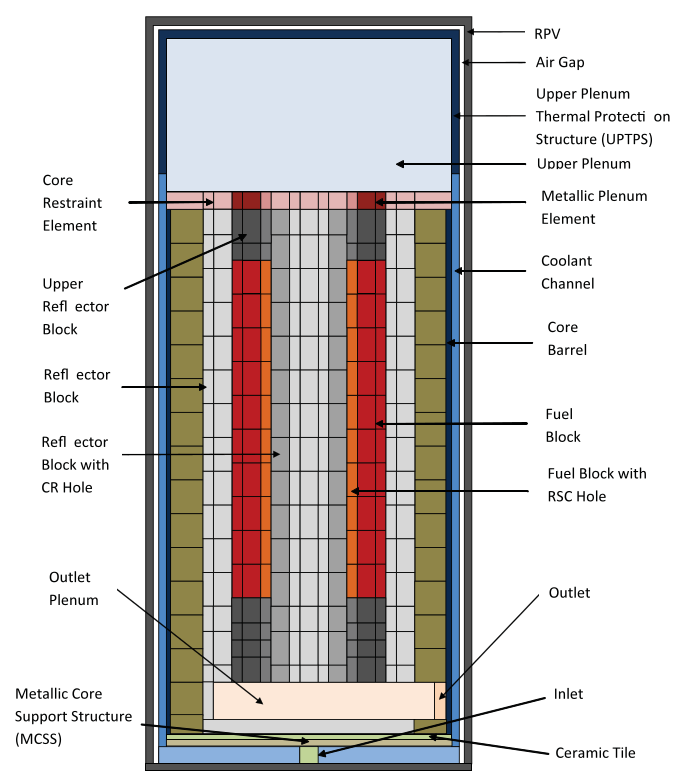
\includegraphics[width=\linewidth]{figures/axial-layout.png}
	% 		\caption{YZ-plane.}
	% 	\end{subfigure}
	% 	\hfill
	% 	\caption{MHTGR reactor layout.}
	% 	\label{fig:layout}
	% \end{figure}

	% \begin{figure}[htbp!]
	% 	\centering
	% 	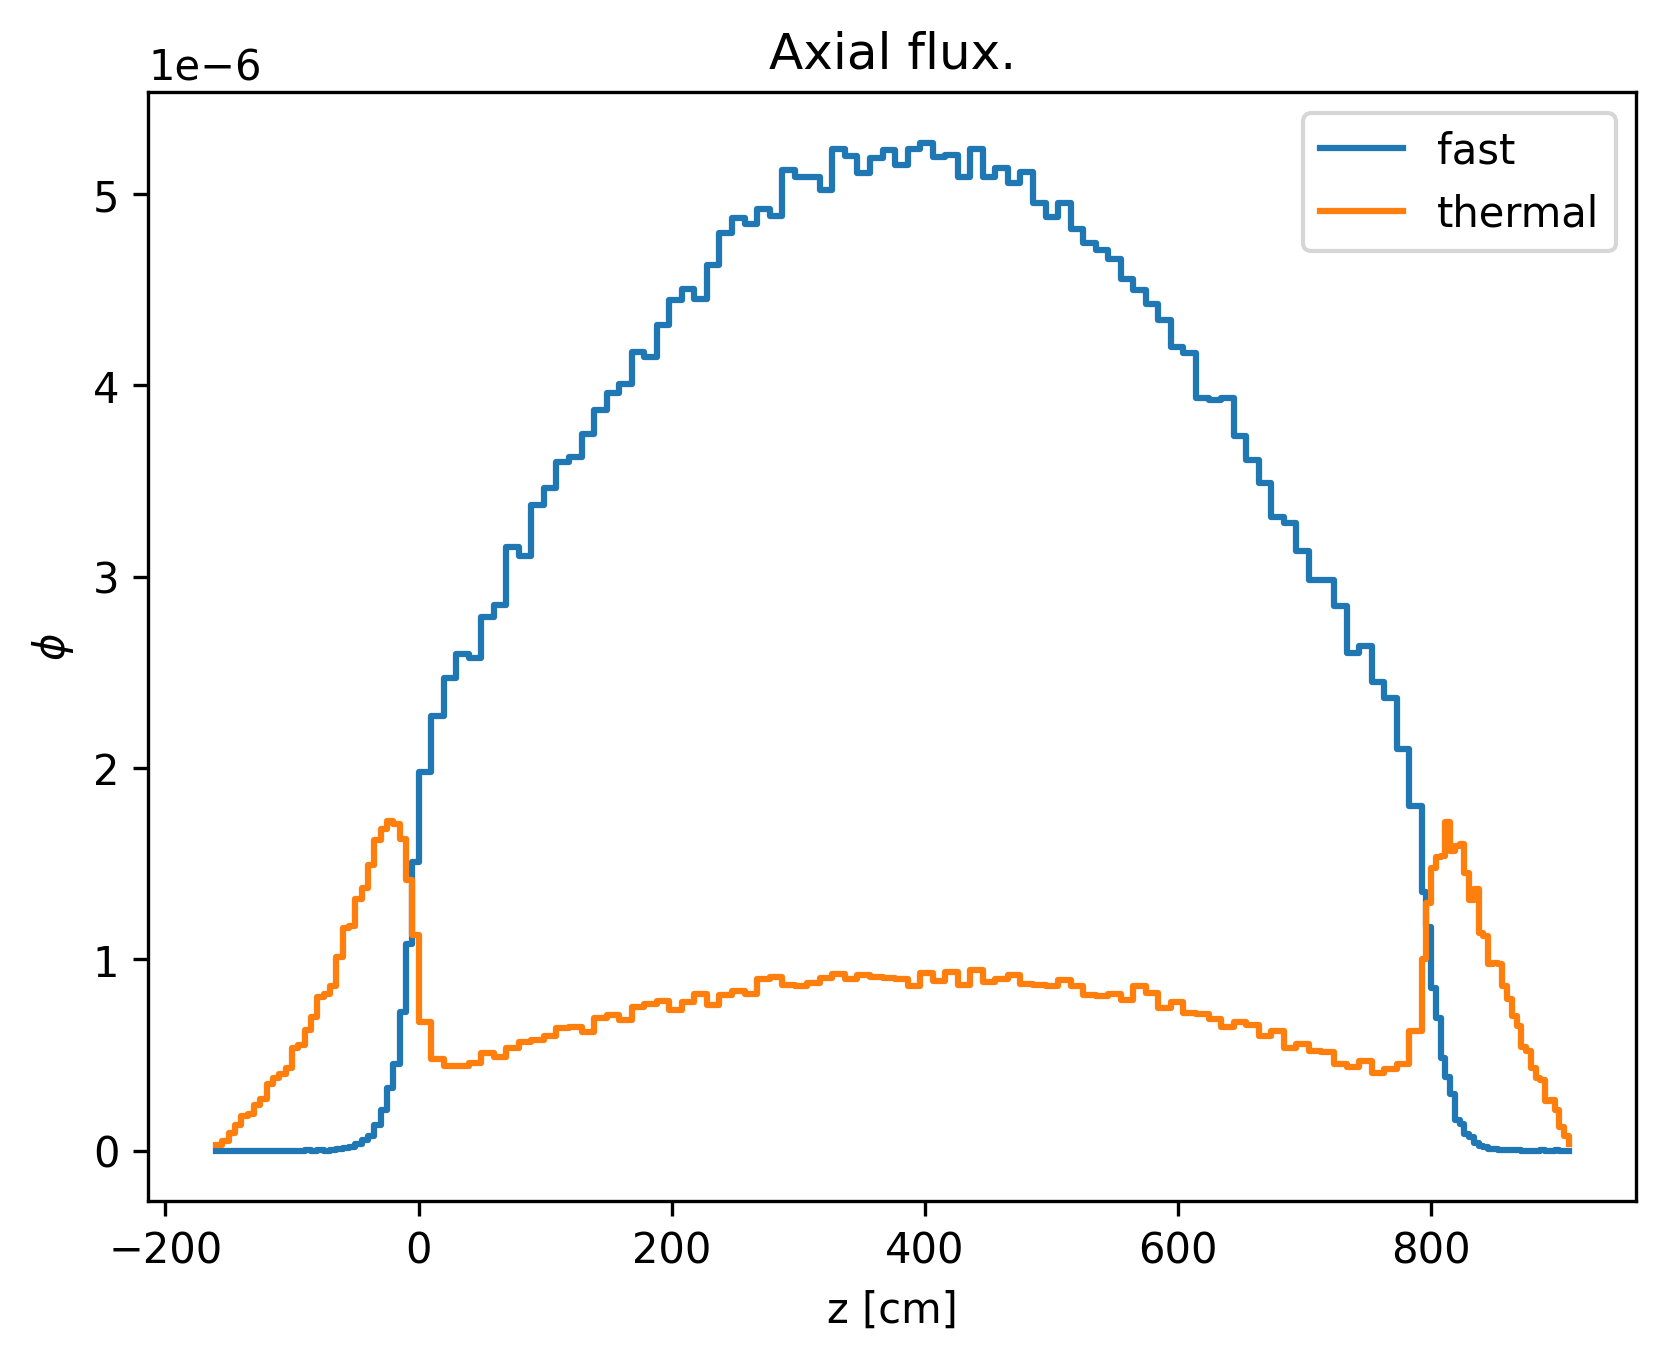
\includegraphics[width=0.6\linewidth]{figures/axial1.png}
	% 	\hfill
	% 	\caption{Neutron flux on the specified fuel channel.}
	% 	\label{fig:axial}
	% \end{figure}